

\newpage



%----------------------------------------------------------------------------------------


\section[Static Correlations][Corrélations Statiques]{Static correlations of urban form and network shape}{Corrélations Statiques entre Forme Urbaine et Forme de Réseau}

\label{sec:staticcorrelations}


%----------------------------------------------------------------------------------------



Une première entrée en matière empirique, et qui se voudra simple sur les objets étudiés, est de s'intéresser à des caractéristiques directement mesurables des territoires et réseaux. De manière phénoménologique, les agrégats urbains se qualifient au dessus d'une certaine échelle par une forme urbaine, de même que les réseaux de transport présentent des propriétés topologiques synthétiques. On peut alors s'interroger sur des liens directement mesurables entre ceux-ci, c'est à dire quelle information contiennent les corrélations statiques entre forme urbaine et topologie du réseau routier, au sens de corrélations estimées sur un échantillon local dans l'espace sur des données fixes. Dans une perspective de la Théorie Evolutive, on devine bien les implications de cette démarche: les liens entre corrélations dynamiques et statiques sont liées aux propriétés d'ergodicité du système, et la variation des estimateurs dans l'espace et selon les échelles informera sur le degré de stationnarité des interactions. Il s'agit d'une manière indirecte de lier statique et dynamique.


\bpar{
Spatio-temporal processes implying diffusion or propagation phenomena generally have a specific structure of correlation. In particular, as derived in section~\ref{sec:spatiotempcorrs}, a static computation of correlation between different instances of a system may under certain conditions provide information on dynamical correlations implied.
}{
Les processus spatio-temporels impliquant une diffusion ou une propagation (ce qui est a priori le cas de la forme urbaine comme suggéré par~\ref{sec:densitygeneration}) peuvent généralement être compris partiellement par leur structure de correlation dans le temps et l'espace. On suggère par exemple en Appendice~\ref{sec:spatiotempcorrs} des cas idéaux pour lesquels un lien peut être directement obtenu. Dans certains cas, on peut espérer que l'étude d'une correlation statique entre différentes instances d'un système peuvent sous certaines conditions informer sur les correlations dynamiques sous-jacentes, ce que nous ferons de manière empirique ici.
}




\bpar{
At the macroscopic scale of system of cities, the spatial nature of the urban system is reasonably captured by cities position, associated with aggregated city variable to represent entirely the system (see e.g. ontologies of Simpop models~\cite{pumain2012multi} or its successor Marius~\cite{cottineau2014evolution}). At the mesoscopic scale at which we aim to capture morphological manifestations of interactions between transportation networks and territories, structure of the territorial system can be specified by more refined indicators for the morphological aspect.
}{
A l'échelle macroscopique du système de ville, le caractère spatial du système urbain est capturé de manière raisonnable par les positions des villes, associées aux variables agrégées au niveau de la ville qui représentent entièrement le système, comme la plupart des modèles liés à la Théorie Evolutive postulent. A l'échelle mesoscopique, à laquelle nous nous attendons à capturer des manifestations morphologiques des interactions entre ville et transport, la structure du système territorial peut être spécifiée par des indicateurs plus raffinés pour l'aspect morphologique. Le choix des indicateurs de forme urbaine pertinents pour répondre à un type de question donnée n'est pas évident, et dépendra de l'échelle et du contexte : on peut par exemple s'intéresser au caractère polycentrique pour lequel les indicateurs seront différents si on s'intéresse à des phénomènes de concentration. Notre but est de capturer le maximum de dimensions de variation de la forme urbaine, nous calculerons pour cela un certain nombre d'indicateurs arbitraire satisfaisant une certaine convergence de la variance cumulée des composantes principales.
}



\bpar{
We study systematically morphological indicators for constant size areas covering a given geographical area. The choice of fixed size areas can be questioned regarding definition of a territorial system, that can be otherwise understood as a consistent spatial entity at a given scale and along certain criteria : \emph{Human territories} as defined by Raffestin (op. cit.) or more generally functionally autonomous spaces\footnote{for example, a tentative of definition of a \textit{Parisian} territory would present many facets. From the subjective territory point of view, intra-muros Parisians consider a strict boundary at \textit{Boulevard Periph{\'e}rique}, whereas close and even further suburbs will be seen as Parisians from the Province. The functional territory of \textit{Metropolitain} extends slightly further than the administrative boundary. Governance perimeters are currently mutating with the Metropolitan governance project. Complementary perceptions of the territory can thus be multiplied.}. Here we choose the mesoscopic scale of a metropolitan center ($\simeq$ 50km) for comparability purposes and because greater scale are no more relevant regarding urban form, whereas smaller scales must contain too much noise. 
}{
Nous étudions de manière systématique les indicateurs morphologiques pour des zones d'aire constante couvrant une région donnée. Le choix de zones de taille fixe peut être interrogé au regard de la définition d'un système territorial, qui peut par ailleurs être compris comme une entité spatiale consistante à une échelle donnée et selon certains critères : les \emph{Territoires Humains} comme nous avons déjà défini en~\ref{sec:networkterritories} ou plus généralement des espace fonctionnels autonomes\footnote{par example, tenter de définir un territoire \emph{Parisien} présenterait plusieurs facettes. Du point de vue du territoire subjectif, les Parisiens intra-muros considèrent une barrière stricte au Boulevard Périphérique, tandis que des banlieues plus ou moins proches seront vues comme parisiennes depuis la province. Le territoire fonctionnel du Métropolitain s'étend légèrement plus loin que la limite administrative de Paris, mais couvre quasiment toute l'Ile-de-France lorsqu'on y ajoute RER et Transilien. Les périmètres de gouvernance sont en train d'évoluer avec le projet de gouvernance métropolitaine (voir~\ref{sec:casestudies}). Des perceptions complémentaires du territoires peuvent ainsi être multipliées.}. Le choix de limites ``pertinentes'' pour le territoire ou la ville est un problème relativement ouvert \cite{guerois2002commune} qui dépendra souvent de la question à laquelle on cherche à répondre. Nous choisissons ici l'échelle mesoscopique d'un centre métropolitain ($\simeq$ 50km) d'une part pour la cohérence du champ spatial calculé, et d'autre part parce que des échelles plus grandes deviennent moins pertinentes pour la notion de forme urbaine, tandis que des échelles plus petites contiennent un bruit trop grand.
}


Le but n'étant pas de comparer les territoires sur lesquels ces indicateurs sont calculés entre eux, mais de calculer une valeur ``locale'' et d'établir un champ discret régulier dans l'espace, la taille fixe de la fenêtre est nécessaire. Cette taille est arbitraire, mais l'analyse a été menée pour des tailles voisines également (voir~\ref{app:sec:staticcorrelations}). Les ``territoires'' qu'une approche plus classique voudra comparer, comme des aires urbaines fonctionnelles par exemple, pourront émerger de manière endogène si ceux-ci font sens pour les variations des indicateurs.





%%%%%%%%%%%%%%%%%%
\subsection{Morphological Measures}{Mesures morphologiques}

\paragraph{Urban Morphology}{Morphologie Urbaine}


\bpar{
\cite{guerois2008built} studies the form of European cities using a simple measure of density slopes from the center to the periphery. We need however quantities having a certain level of robustness and invariance. For example, two polycentric cities should be classified as morphologically close whereas a direct comparison of distributions (with the Earth Mover Distance for example) could give a very high distance between configurations depending on center positions. The use of fractal indexes is a possibility suggested by~\cite{2016arXiv160808839C}. We choose to refer to the literature in Urban Morphology which proposes an extensive set of indicators to describe urban form~\cite{tsai2005quantifying}. The number of dimensions can be reduced to obtain a robust description with a few number of independent indicators~\cite{Schwarz201029}. Note that here we consider indicators on population density only, and that more elaborated considerations on Urban Form include for example the distribution of economic opportunities and the combination of these two fields through accessibility measures. For the choice of indicators, we follow the analysis done in~\cite{le2015forme} in which a morphological typology of large european cities is obtained.
}{
\cite{guerois2008built} étudie la forme des villes Européennes par l'utilisation d'une mesure simple des gradients de densité du centre vers la périphérie. Nous avons cependant besoin de mesures ayant un certain niveau de robustesse et d'invariance. Par exemple, deux villes polycentriques devraient être classifiées comme morphologiquement proches tandis qu'une comparaison directe des distributions (avec une distance de Monge par exemple) pourra donner une distance très élevée entre les configurations selon la position des centres. L'utilisation d'indices issus de l'analyse fractale est une possibilité suggérée par~\cite{2016arXiv160808839C}. Le lien entre morphologie urbaine et topologie du graphe de relations correspondant a été suggéré par\cite{badariotti2007conception}. Nous choisissons de nous référer à la littérature en morphologie urbaine qui propose des jeux d'indicateurs variés pour décrire la forme urbaine~\cite{tsai2005quantifying}. Le nombre de dimensions peut être réduit pour obtenir une description robuste avec un petit nombre d'indicateurs indépendants~\cite{Schwarz201029}. Il faut noter que nous ne considérons ici des indicateurs sur la densité de population seule, et que des considérations plus élaborées sur la forme urbaine incluent par exemple la distribution des opportunités économiques et la combinaison de ces deux champs par des mesures d'accessibilité. Pour le choix des indicateurs, nous suivons l'analyse faite dans~\cite{le2015forme} où une typologie morphologique des grandes villes européennes est obtenue.
}

\bpar{
We give now the formal definition of morphological indicators. We consider gridded population data $(P_i)_{1\leq i \leq N^2}$, write $M=N^2$ the number of cells, $d_{ij}$ the distance between cells $i,j$, and $P=\sum_{i=1}^{M} P_i$ total population. We measure Urban Form using:

\begin{enumerate}
\item Rank-size slope $\gamma$, expressing the degree of hierarchy in the distribution, computed by fitting with Ordinary Least Squares a power law distribution by $\ln \left( P_{\tilde{i}}/P_0\right) \sim k + \gamma\cdot \ln \left(\tilde{i}/i_0\right)$ where $\tilde{i}$ are the indexes of the distribution sorted in decreasing order. It is always negative, and values close to zero mean a flat distribution.
\item Entropy of the distribution, that expresses how uniform the distribution is:
\begin{equation}
\mathcal{E} = \sum_{i=1}^{M}\frac{P_i}{P}\cdot \ln{\frac{P_i}{P}}
\end{equation}
$\mathcal{E}=0$ means that all the population is in one cell whereas $\mathcal{E}=0$ means that the population is uniformly distributed.
\item Spatial-autocorrelation given by Moran index, with simple spatial weights given by $w_{ij} = 1/d_{ij}$
\[
I = \frac{\sum_{i\neq j} w_{ij} \left(P_i - \bar{P}\right)\cdot\left(P_j - \bar{P}\right)}{\sum_{i\neq j} w_{ij} \sum_{i}{\left( P_i - \bar{P}\right)}^2}
\]
Positive values will imply aggregation spots (``density centers''), negative values strong local variations whereas $I=0$ corresponds to totally random population values.
\item Mean distance between individuals, which captures population concentration
\[
\bar{d} = \frac{1}{d_M}\cdot \sum_{i<j} \frac{P_i P_j}{P^2} \cdot d_{ij}
\]
where $d_M$ is a normalisation constant taken as the diagonal of the world in our case.
\end{enumerate}
}{
Nous donnons à présent une définition formelle des indicateurs morphologiques. Nous considérons des données de population en grille $(P_i)_{1\leq i \leq N^2}$, écrivons $M=N^2$ le nombre de cellules, $d_{ij}$ la distance entre les cellules $i,j$, et $P=\sum_{i=1}^{M} P_i$ la population totale. La forme urbaine est mesurée par : 

\begin{enumerate}
\item Pente de la loi rang-taille $\gamma$, qui exprime le degré de hiérarchie de la distribution, calculé en ajustant une loi de puissance par Moindres Carrés Ordinaires par $\ln \left( P_{\tilde{i}}/P_0\right) \sim k + \gamma\cdot \ln \left(\tilde{i}/i_0\right)$ où $\tilde{i}$ sont les indices de la distribution triée de manière décroissante. Elle est toujours négative, et des valeurs proches de zéro signifient une distribution plate.
\item Entropie de la distribution, qui exprime l'uniformité de la distribution:
\begin{equation}
\mathcal{E} = \sum_{i=1}^{M}\frac{P_i}{P}\cdot \ln{\frac{P_i}{P}}
\end{equation}
$\mathcal{E}=0$ signifie que toute la population est dans une cellule tandis que $\mathcal{E}=0$ signifie que la population est distribuée uniformément.
\item L'auto-corrélation spatiale donnée par l'indice de Moran, avec des poids spatiaux simples donnés par $w_{ij} = 1/d_{ij}$
\[
I = \frac{\sum_{i\neq j} w_{ij} \left(P_i - \bar{P}\right)\cdot\left(P_j - \bar{P}\right)}{\sum_{i\neq j} w_{ij} \sum_{i}{\left( P_i - \bar{P}\right)}^2}
\]
Des valeurs positives impliques des lieux d'agrégation (``centres de densité''), des valeurs négatives des fortes variations locales, tandis que $I=0$ correspond à des valeurs de population totalement aléatoires.
\item Distance moyenne entre individus, qui capture la concentration de la population
\[
\bar{d} = \frac{1}{d_M}\cdot \sum_{i<j} \frac{P_i P_j}{P^2} \cdot d_{ij}
\]
où $d_M$ est une constante de normalisation que nous prenons comme la diagonale de l'étendue considérée dans notre cas.
\end{enumerate}
}

Les deux premiers indexes ne sont pas spatiaux, mais nécessaires pour une bonne qualification des distributions de population, et sont complétés par les deux derniers prenant en compte l'espace.


%%%%%%%%%%%%%%%%%%%%%%%%
\paragraph{Results}{Résultats}



%%%%%%%%%%%%%%%%%%%%%%%%
\begin{figure}
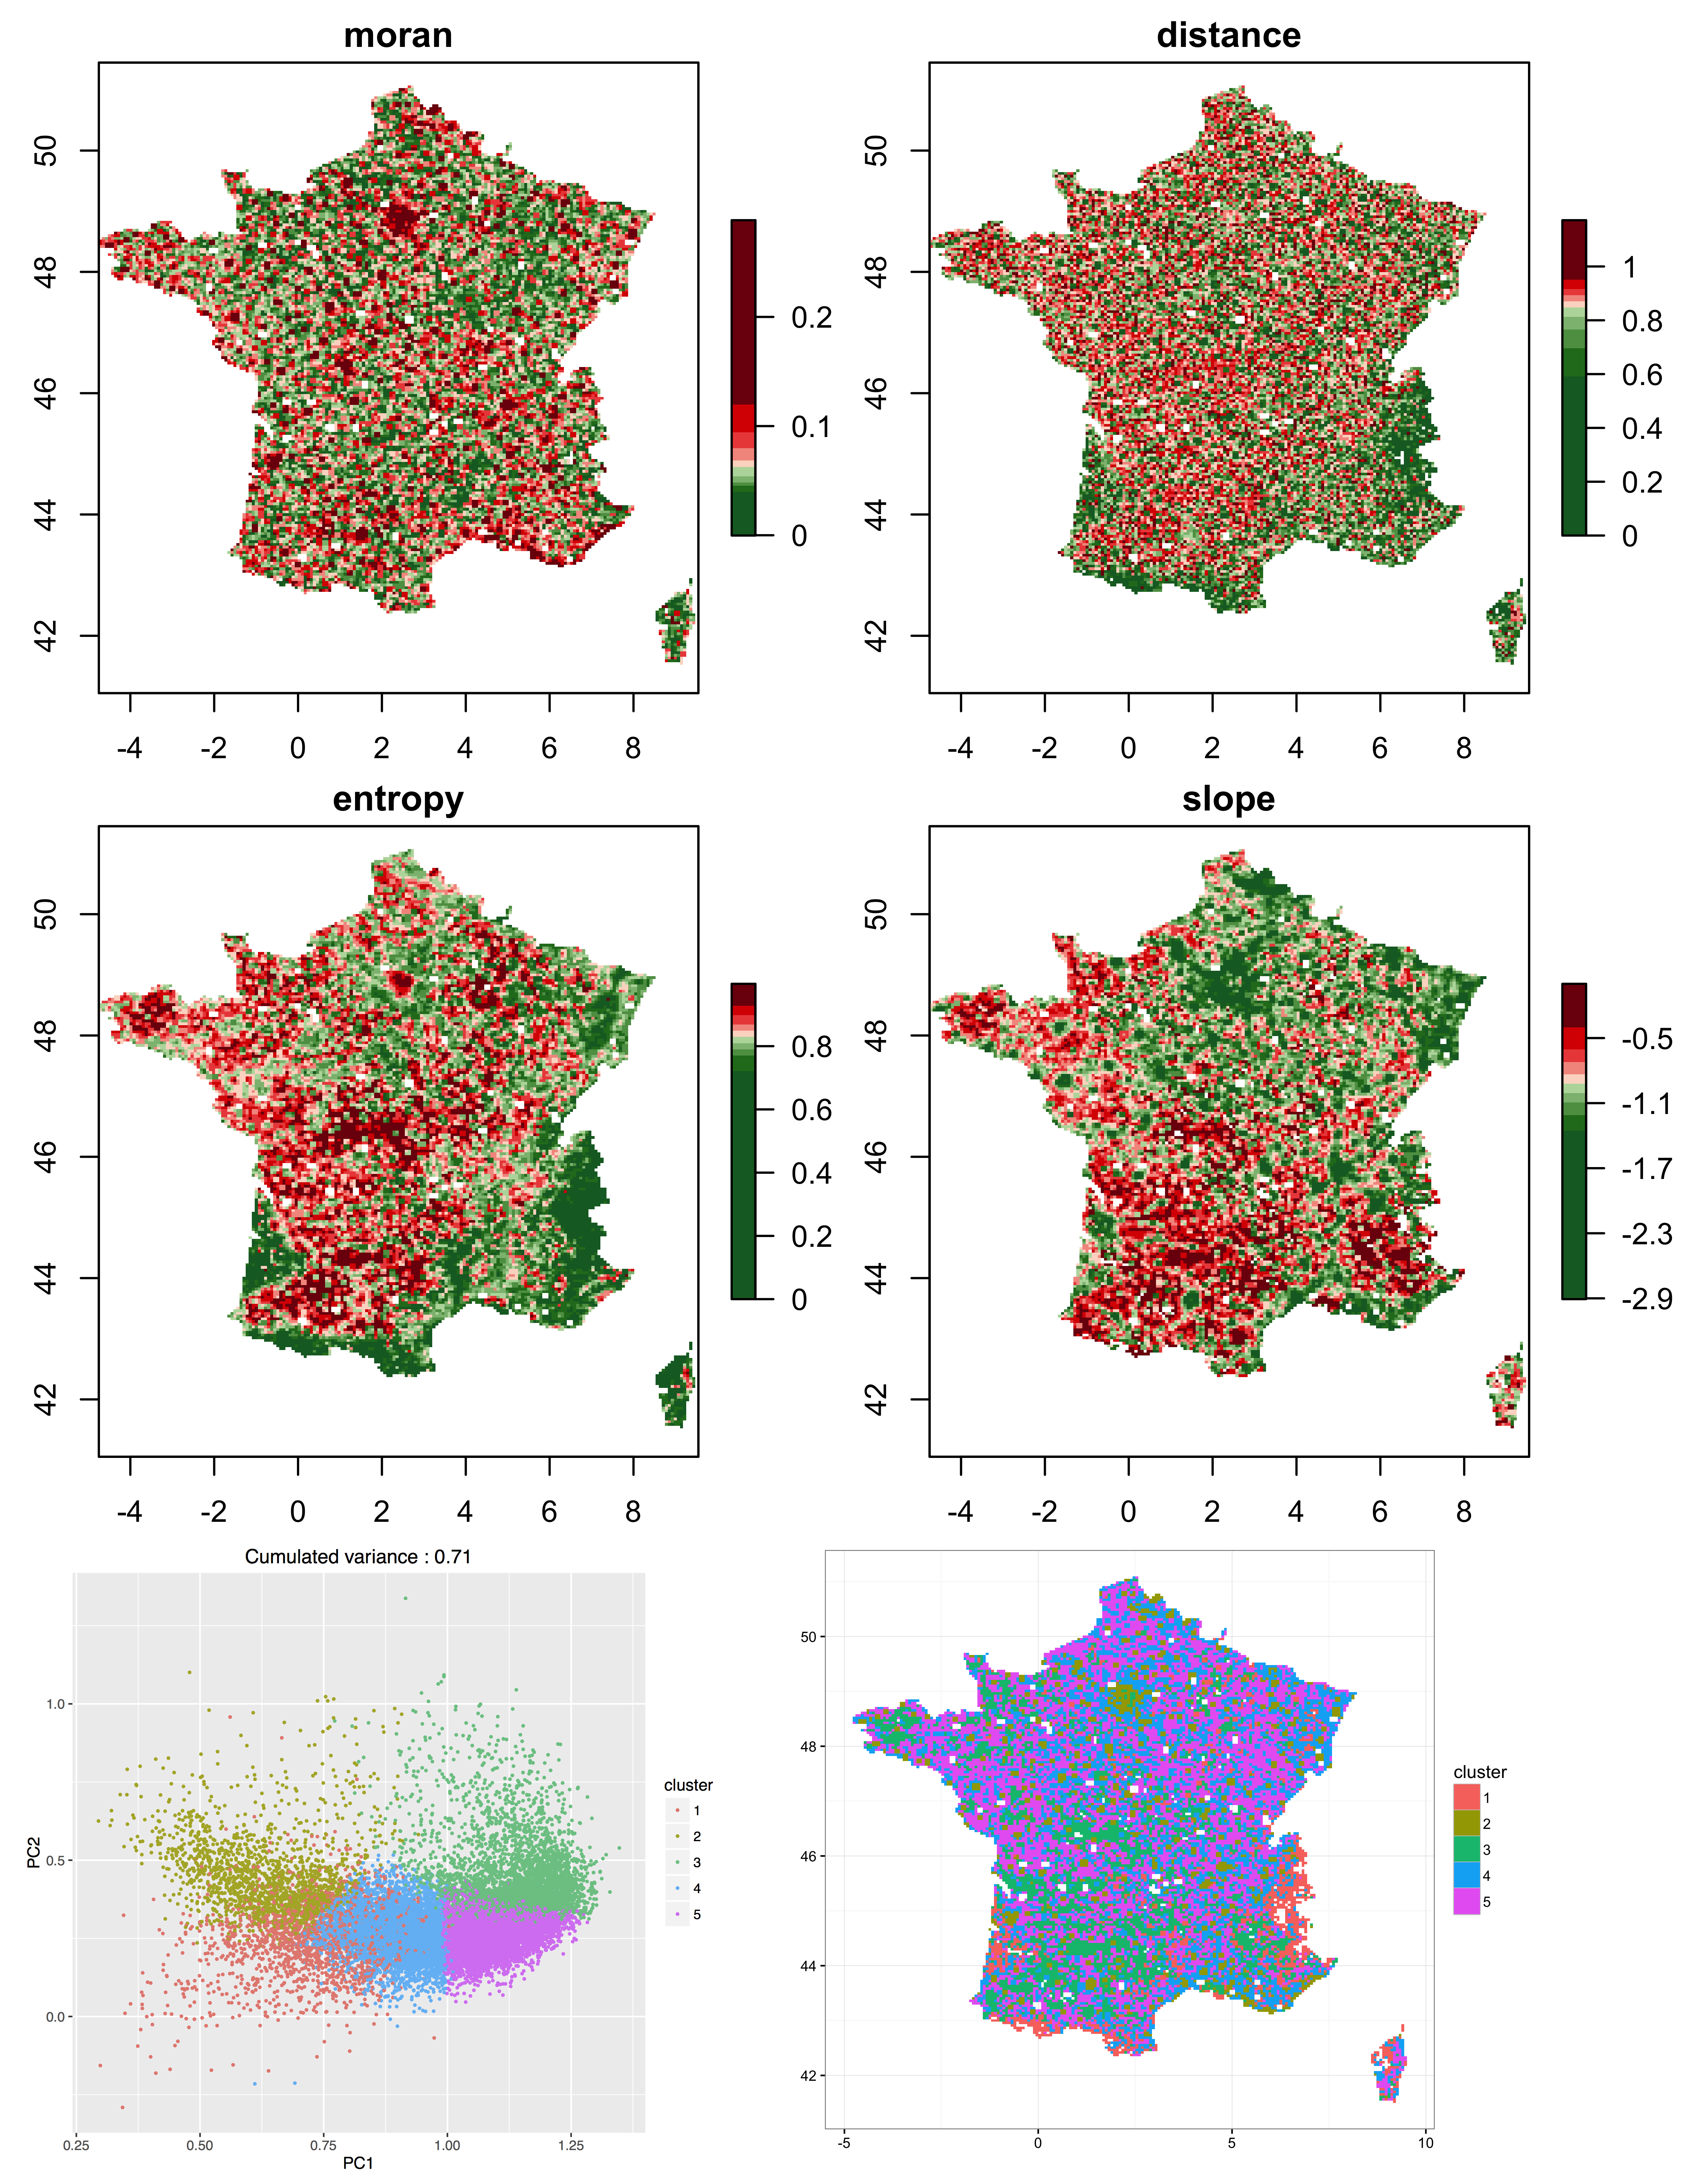
\includegraphics[width=0.9\linewidth]{Figures/Density/Fig1}
%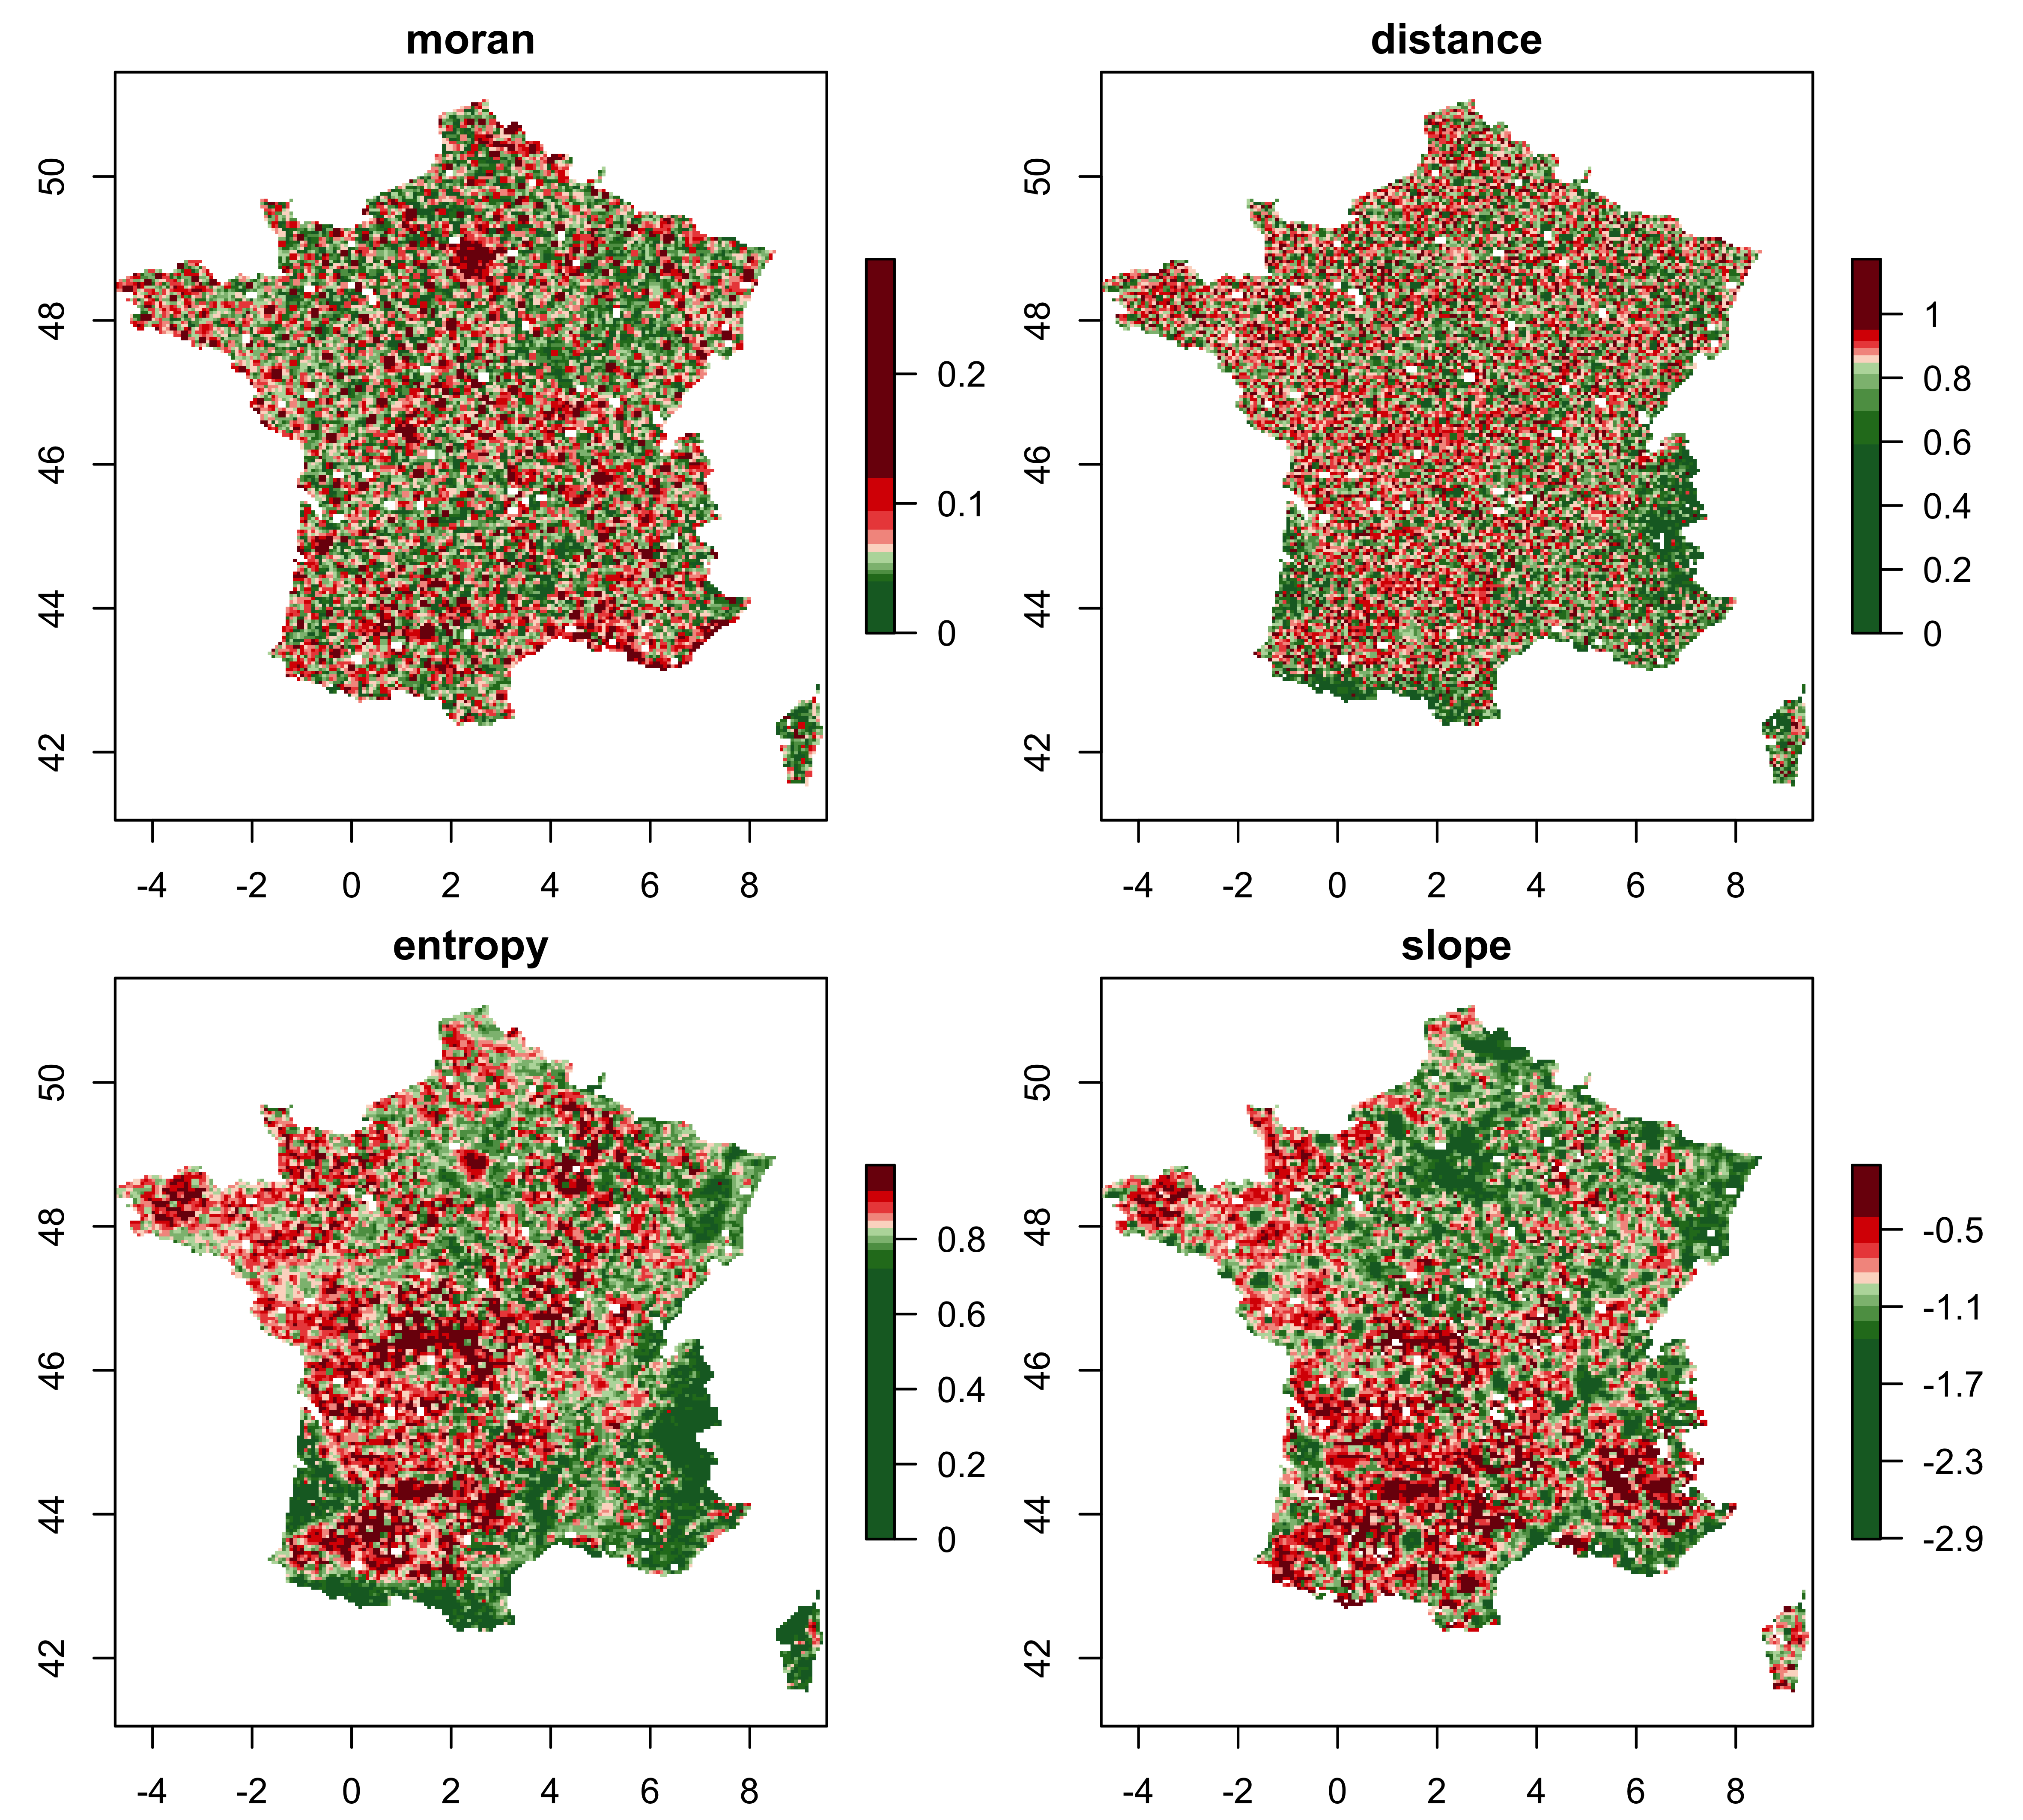
\includegraphics[width=\textwidth]{figures/indics_morpho_discrquantiles}\\
%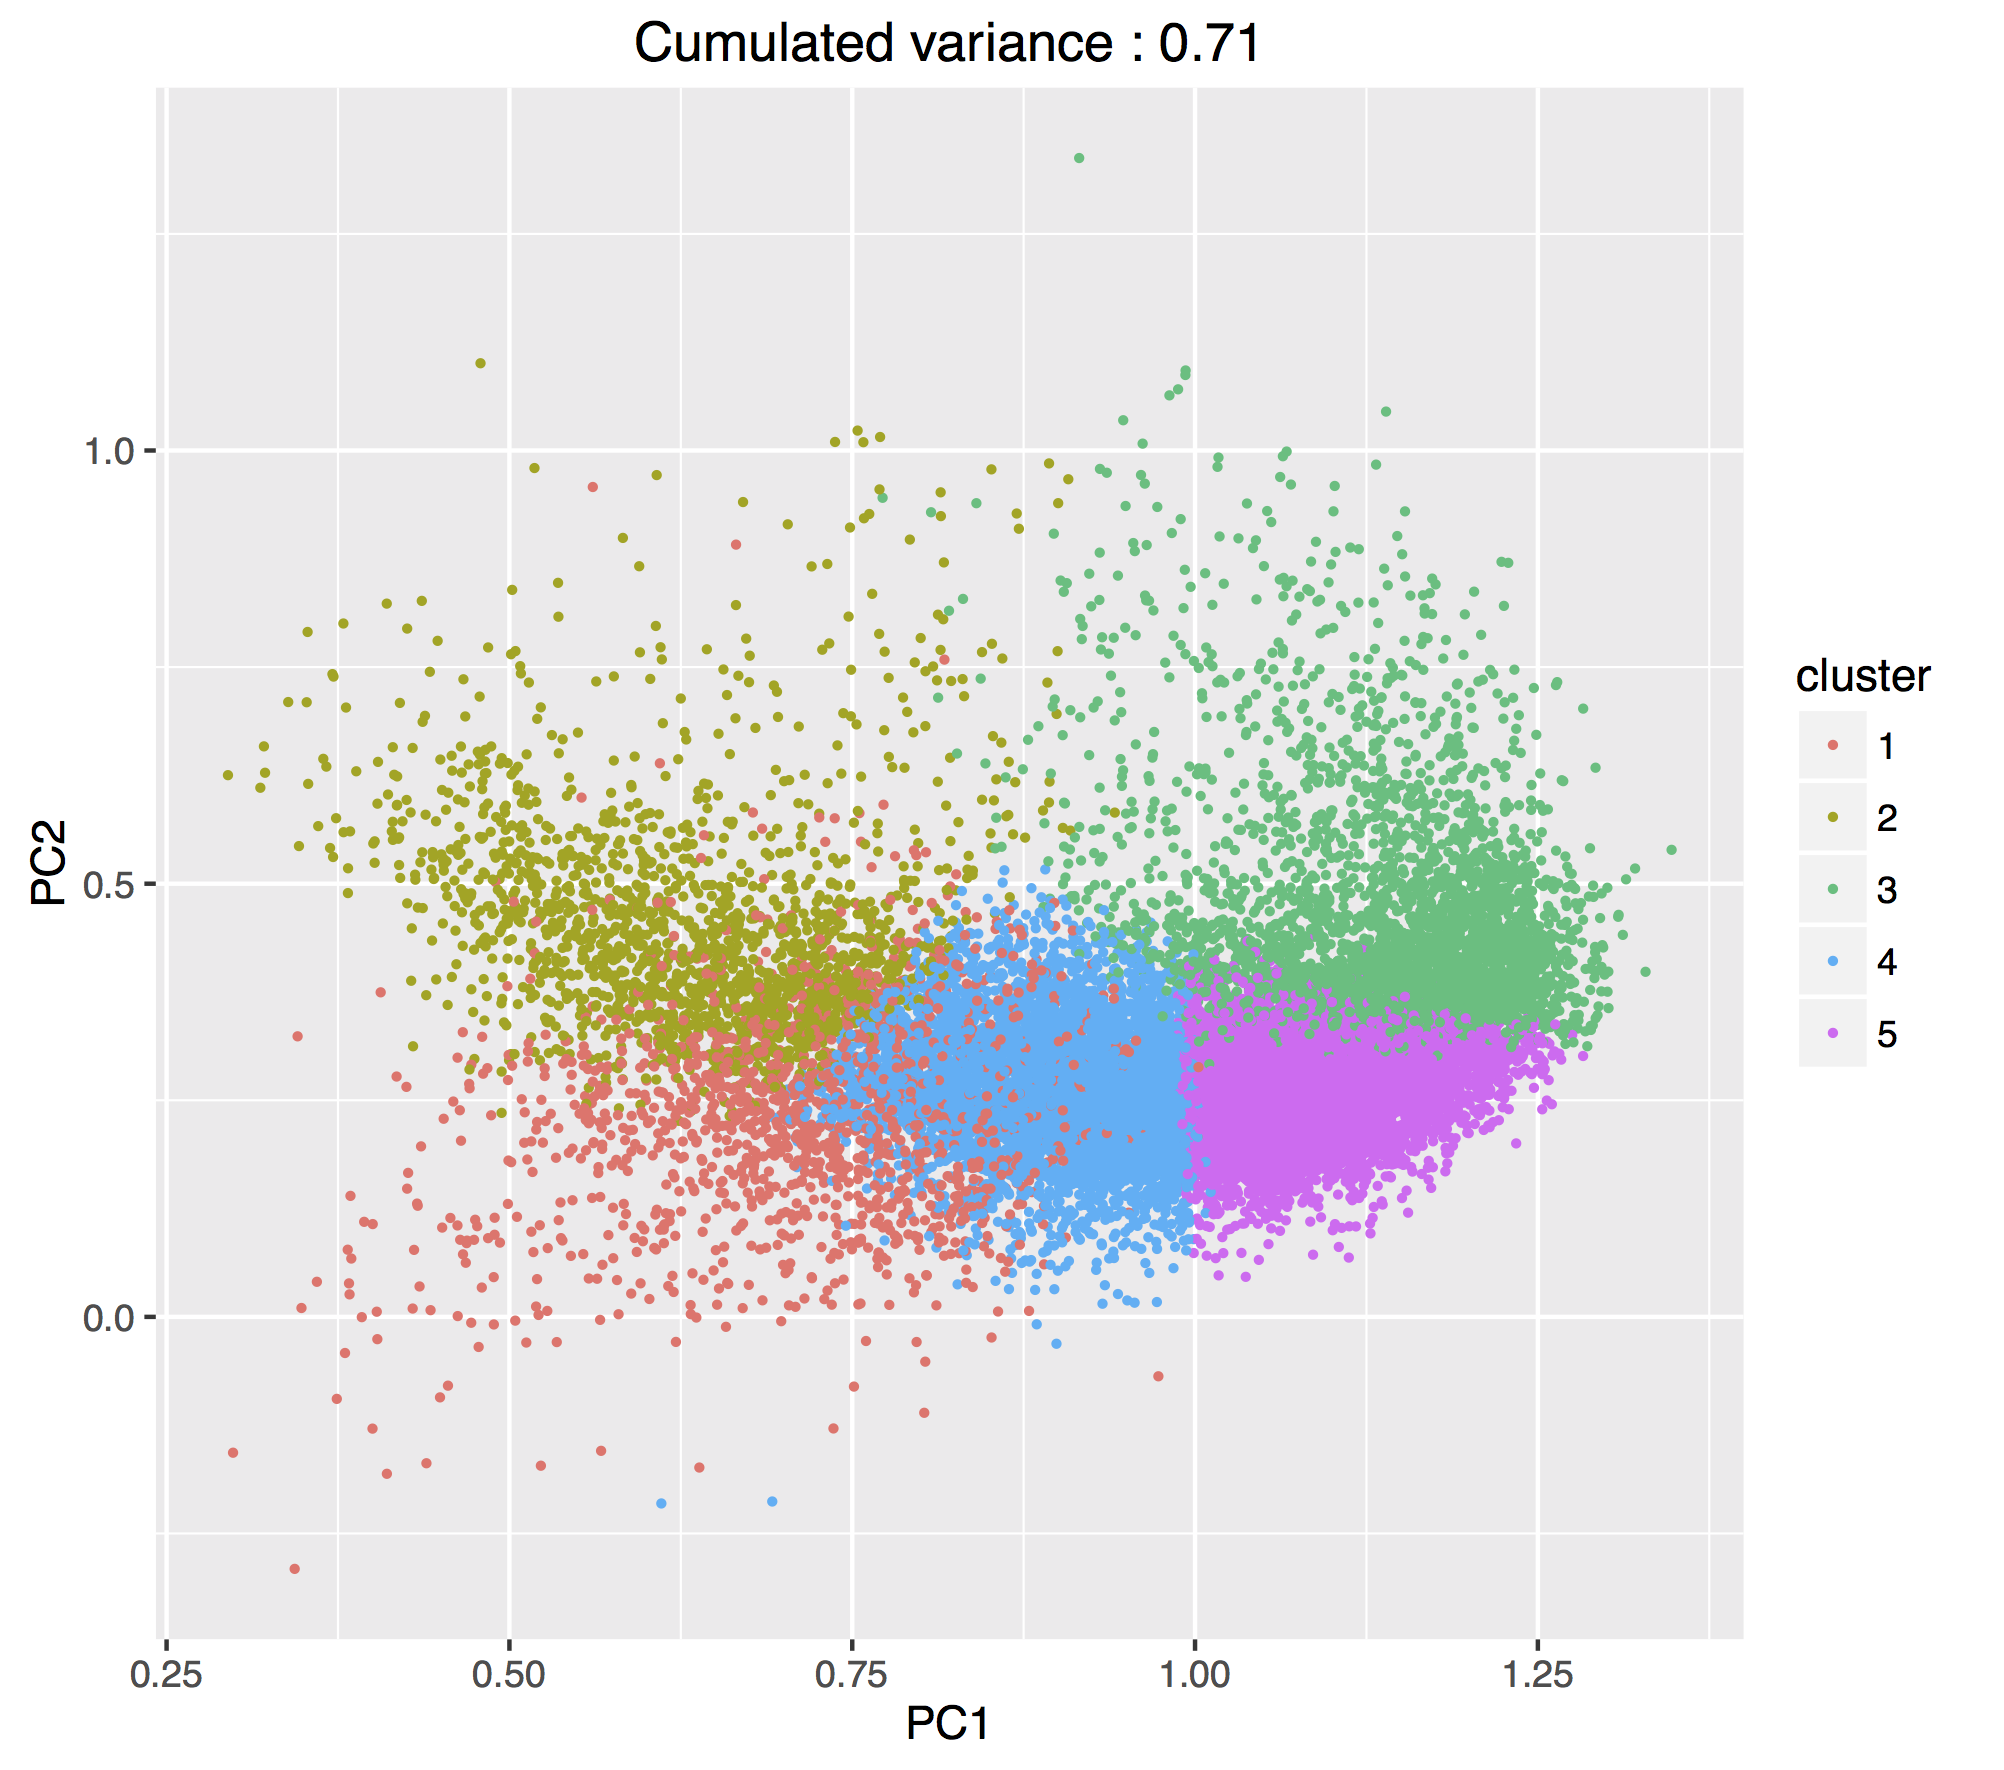
\includegraphics[width=0.49\textwidth]{figures/cluster_pca_k5_morpho}
%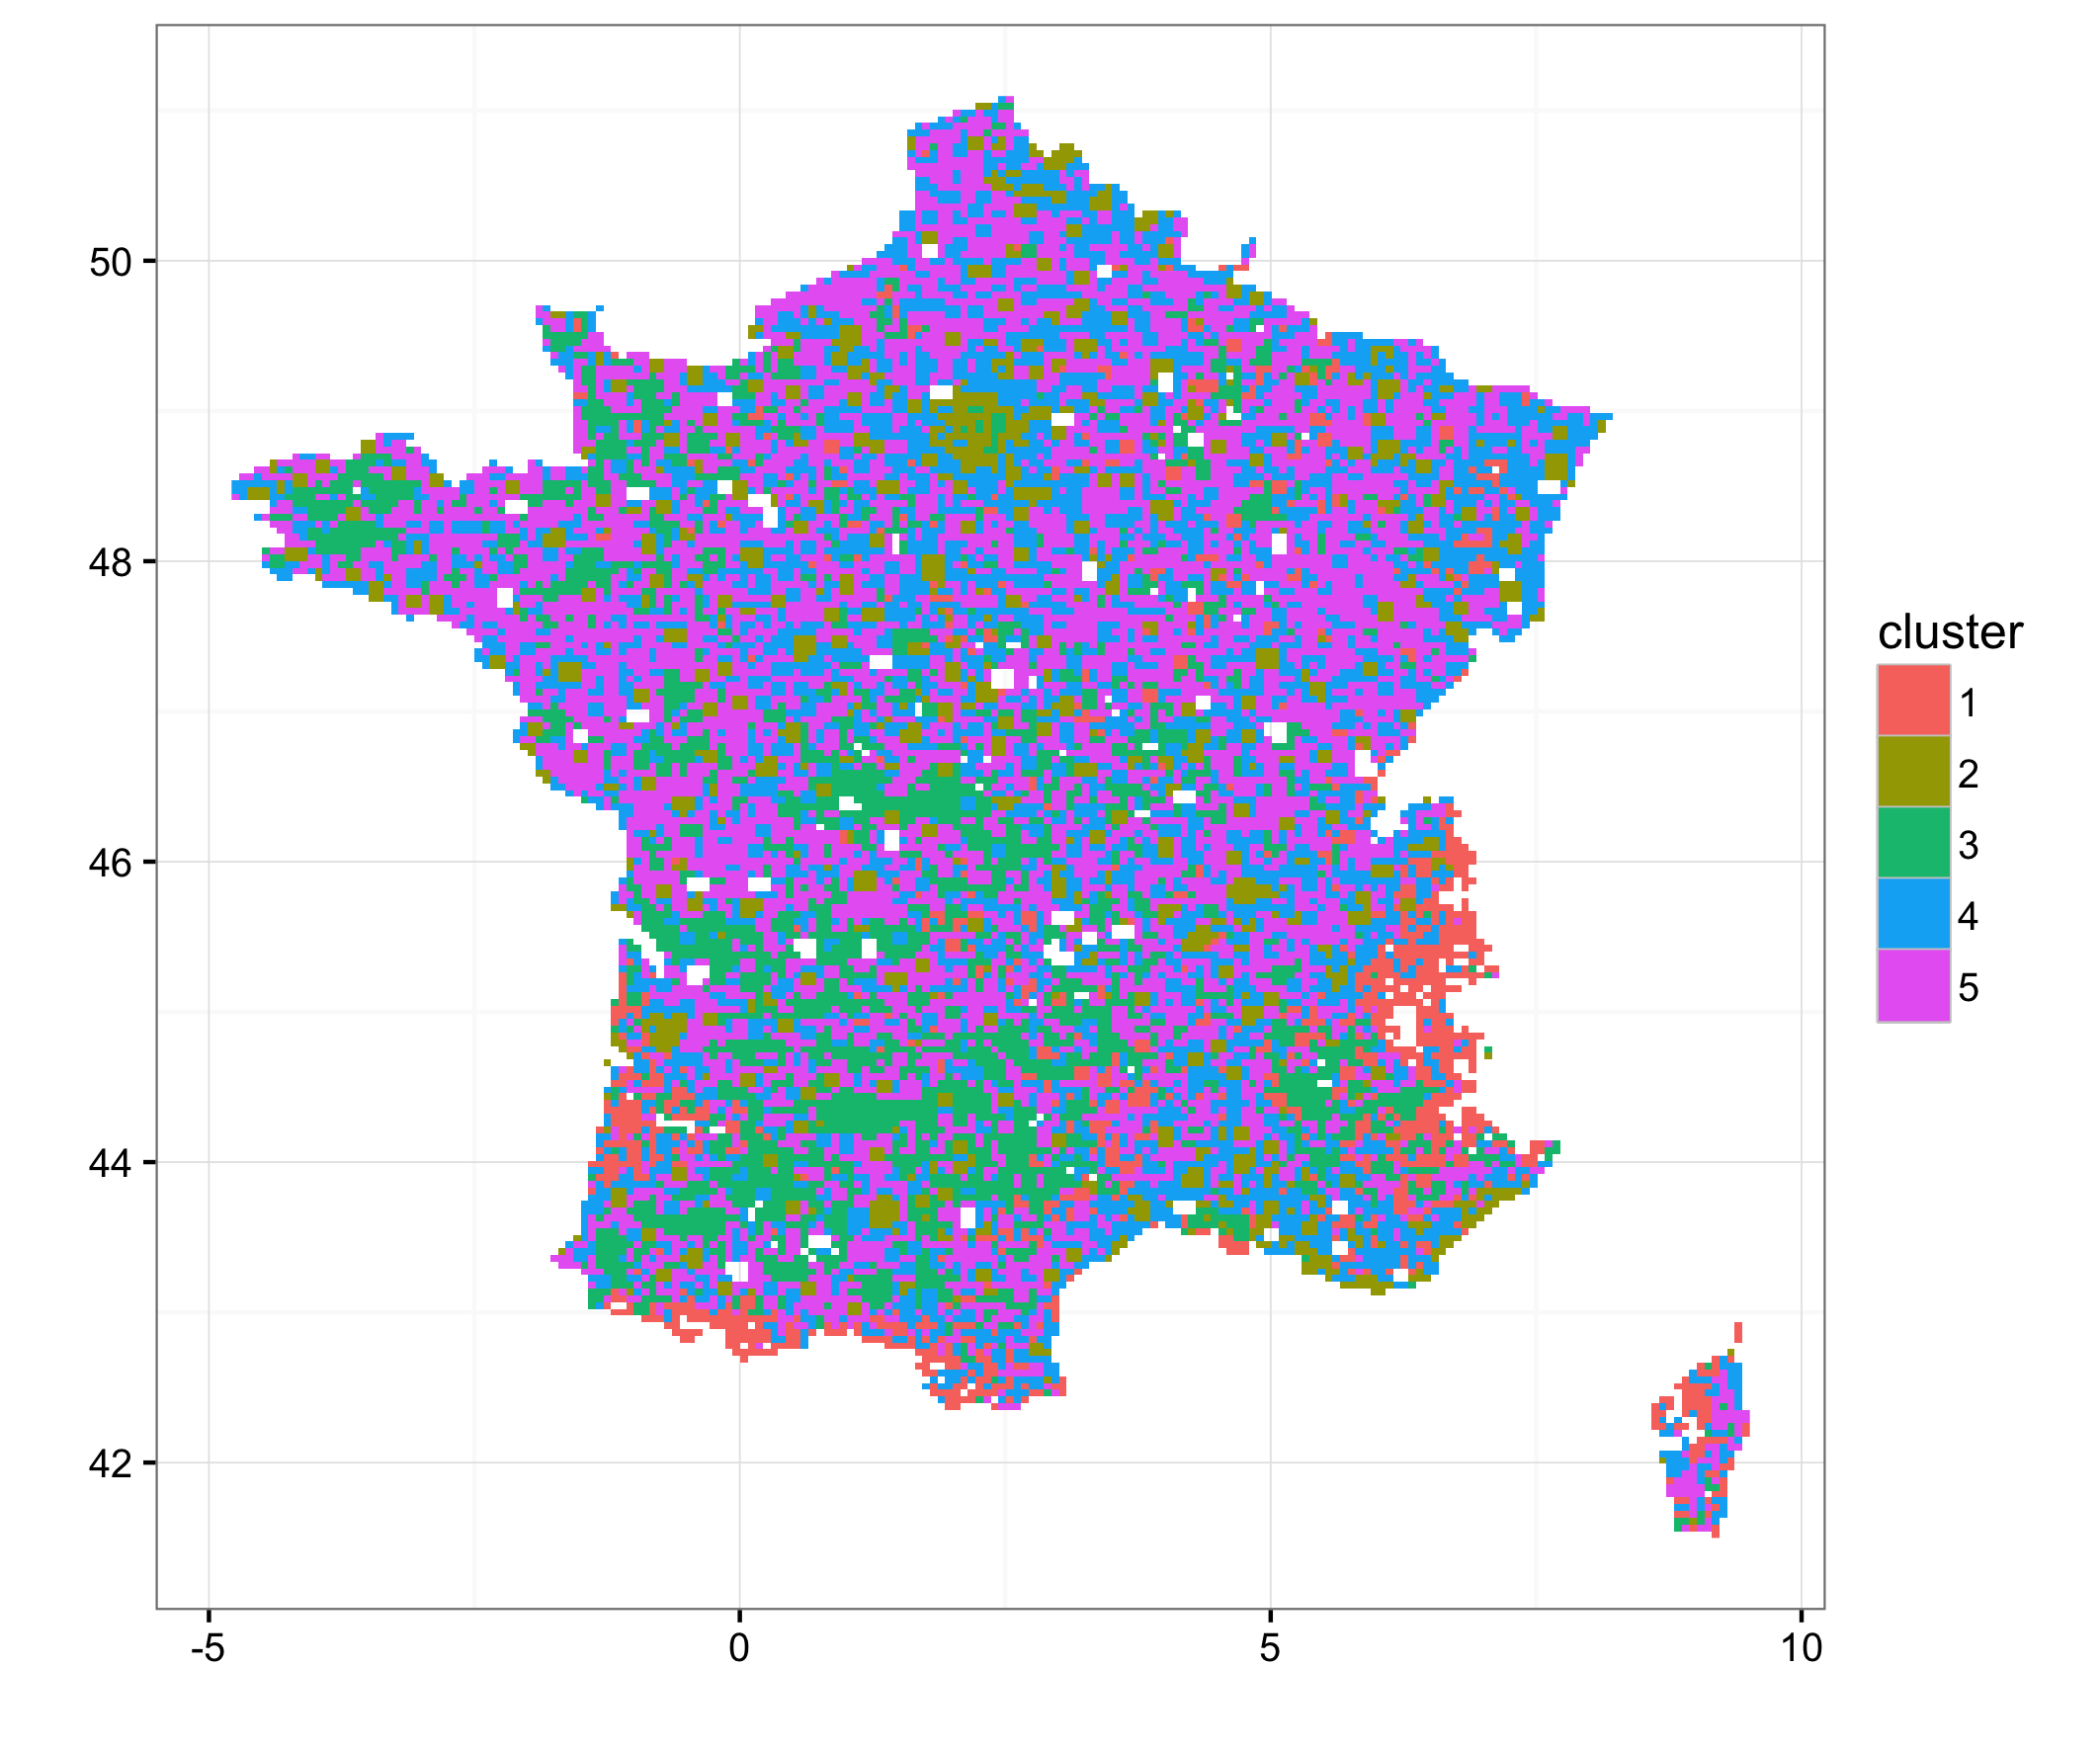
\includegraphics[width=0.49\textwidth]{figures/cluster_map_k5_morpho}
\caption[Empirical values of morphological indicators][Distribution spatiale des morphologies]{\textbf{Empirical values of morphological indicators.} \textit{(Top four maps)} Spatial distribution of the morphological indicators for France. Scale color discretization is done using quantiles to ease map readability. \textit{(Bottom Left)} Projection of morphological values on the two first components on a Principal Component analysis. Color gives cluster in an unsupervised classification (see text). \textit{(Bottom right)} Spatial distribution of clusters.\label{fig:staticcorrelations:empirical}}{\textbf{Valeurs empiriques des indicateurs morphologiques.} \textit{(Quatre cartes du haut)} Distribution spatiale des indicateurs morphologiques pour la France. La détermination de l'échelle de couleur est faite par quantiles pour faciliter la lecture des cartes. \textit{(Bas gauche)} Projection des valeurs morphologiques sur les deux premières composantes d'une analyse en composantes principales. La couleur donne le cluster dans une classification non supervisée (voir texte). \textit{(Bas droite)} Distribution spatiale des clusters.\label{fig:staticcorrelations:empirical}}
\end{figure}
%%%%%%%%%%%%%%%%%%%%%%%%



\bpar{
We compute the morphological measures given above on real urban density data, using the population density grid of the European Union at 100m resolution provided openly by Eurostat~\cite{eurostat}. The choice of the resolution, the spatial range, and the shape of the window on which indicators are computed, is made according to the thematic specifications given before. We consider 50km wide square windows to be in accordance with the expected spatial range of one model instance. As it also does not make sense to have a too detailed resolution because of data quality, we take $N=100$ and aggregate the initial raster data at a 500m resolution to meet this size on real windows. To have a rather continuous distribution of indicators in space, we overlap windows by setting an offset of 10km between each, what also somehow rules out the question of window shape bias by the ``continuity'' of values. We tested the sensitivity to window size by computing samples with 30km and 100km window sizes and obtained rather similar spatial distributions. We show in Fig.~\ref{fig:staticcorrelations:empirical} maps giving values of indicators for France only to ease maps readability. The first striking feature is the diversity of morphological patterns across the full territory. The auto-correlation is naturally high in Metropolitan areas, with the Parisian surroundings clearly detached. When looking at other indicators, it is interesting to denote regional regimes: rural areas have much less hierarchy in the South than in the North, whereas the average distance is rather uniformly distributed except for mountain areas. Regions of very high entropy are observed in the Center and South-West. To have a better insight into morphological regimes, we use unsupervised classification with a simple k-means algorithm, for which the number of clusters $k=5$ witnesses a transition in inter-cluster variance. The split between classes is plotted in Fig.~\ref{fig:empirical}, bottom-left panel, where we show measures projected on the two first components of a Principal Component Analysis (explaining 71\% of variance). The map of morphological classes confirms a North-South opposition in a background rural regime (clear green against blue), the existence of mountainous (red) and metropolitan (dark green) regimes. Such a variety of settlements forms will be the target for the model. We did similar analysis for China using the gridded population data from~\cite{fu1km}: maps are available in~\ref{app:sec:staticcorrelations}.
}{
Nous calculons les mesures morphologiques données ci-dessus sur des données réelles de densité, en utilisant la grille de population de l'Union Européenne à la résolution de 100m fournie de manière ouverte par Eurostat~\cite{eurostat}. Cette base a certains défauts de précision qui ont été reconnus~\cite{bretagnolle2016ville} mais nous agrégerons les données à un niveau suffisant pour les éviter. Le choix de la résolution, de la portée spatiale, et de la forme de la fenêtre sur laquelle les indicateurs sont calculés, sont faits suivant les spécifications thématiques précédentes. Nous considérons des fenêtres carrées de largeur 50km, ce qui permet de plus d'être en accord avec l'ontologie du modèle de morphogenèse que l'on développera en~\ref{sec:densitygeneration}. Comme cela ne fait pas sens d'avoir une résolution trop détaillée à cause de la qualité des données, nous agrégeons les données raster initiales à une résolution de 500m pour avoir des fenêtres de taille $N=100$. Pour obtenir une distribution des indicateurs relativement continue dans l'espace, nous superposons les fenêtres en posant un décalage de 10km entre chaque, ce qui d'une certaine façon résout le problème du biais de la forme de la fenêtre par la ``continuité'' des valeurs. Nous avons testé la sensibilité à la taille de la fenêtre en calculant des échantillons avec des tailles de 30km et 100km et avons obtenu des distributions spatiales assez similaires. L'implémentation des indicateurs doit être faite avec attention, puisque les complexités computationnelles peuvent atteindre $O(N^4)$ pour l'indice de Moran par exemple: nous utilisons les implémentations en \texttt{R} de la convolution par Transformée de Fourier Rapide. Nous montrons en Fig.~\ref{fig:staticcorrelations:empirical} des cartes donnant les valeurs des indicateurs, pour la France seulement afin de permettre une lisibilité. Pour avoir une idée des valeurs typiques de chacun des indicateurs, on pourra se référer aux distributions empiriques données en Appendice~\ref{app:sec:staticcorrelations}. La première caractéristique frappante est la diversité des motifs morphologiques au travers de l'ensemble du territoire. L'auto-correlation est relativement haute dans les zones métropolitaines, avec les environs de Paris qui se détachent clairement. Lorsqu'on s'intéresse aux autres indicateurs, il est intéressant de constater des régimes régionaux: les zones rurales ont beaucoup moins de hiérarchie dans le Sud que dans le Nord, tandis que la distance moyenne est plutôt distribuée uniformément sauf dans les zones montagneuses. Des régions à très forte entropie sont observées dans le centre et le Sud-ouest. Pour avoir une meilleure compréhension des régimes morphologiques, nous utilisons une classification non-supervisée avec un algorithme des k-means simple, pour lequel le nombre de clusters $k=5$ induit une transition dans la variance inter-cluster. La séparation entre les classes est montrée en~\ref{fig:staticcorrelations:empirical}, panneau bas gauche, où nous représentons les mesures projetées sur les deux premières composantes d'une Analyse en Composantes Principales (expliquant 71\% de la variance, ce qui est relativement conséquent). La carte des classes morphologiques confirme une opposition Nord-Sud dans le régime rural de fond (vert clair contre bleu), l'existence d'un régime de montagne (rouge) et d'un régime métropolitain (vert sombre). Une telle variété d'établissements sera l'un des objectifs du modèle en~\ref{sec:densitygeneration}. Un calcul similaire des indicateurs morphologiques a été effectué pour la Chine en utilisant la grille de population à 1km fournie par~\cite{fu1km}. Les cartes sont disponibles en Appendice~\ref{app:sec:staticcorrelations}.
}






%%%%%%%%%%%%%%%%%%
\subsection{Network Measures}{Mesures de Réseau}


\bpar{
We consider network aggregated indicators as a way to characterize transportation network properties on a given territory, the same way morphological indicators yielded information on urban structure. We propose to compute some simple indicators on same extents as for morphology, to be able to explore relations between these static measures. Static network analysis has been extensively documented in the literature, see for example \cite{louf2014typology} for a cross-sectional study of cities or \cite{2015arXiv151201268L} for exploration of new measures for the road network.
}{
Nous considérons d'autre part les mesures agrégées de réseau comme un moyen de caractériser les propriétés des réseaux de transport sur un territoire donné, de la même façon que les indicateurs morphologiques informent sur la structure urbaine. Nous proposons de calculer des indicateurs simples sur des étendues spatiales similaires à la morphologie, pour être en mesure d'explorer les relations entre ces mesures statiques. L'analyse statique de réseau a été intensément documentée dans la littérature, voir par example \cite{louf2014typology} pour une étude comparative des villes ou \cite{2015arXiv151201268L} pour l'exploration de nouvelles mesures pour le réseau de rues.
}


\subsubsection{Data preprocessing}{Pré-traitement des données}


\bpar{
We work here with the road network, which structure is finely conditioned to territorial configuration of population densities. Furthermore, data for present day road network is openly available through the OpenStreetMap project~\cite{openstreetmap}. Its quality was investigated for different countries such as England~\cite{haklay2010good} and France~\cite{girres2010quality}. It was found to be of a quality equivalent to official surveys for the primary road network. Concerning China, although \cite{zheng2014assessing} underlined a quick acceleration of OpenStreetMap road data completeness and accuracy, its use for computation of network indicators may be questioned at a very fine scale. \cite{zhang2015density} highlights four regimes of data quality, partitioning China into regions among which qualitative behavior of OSM data varies. We underline that the results will be more valid on the regions where the quality is the highest, i.e. with high density and high diversity.
}{
Nous travaillons ici avec le réseau de rues, dont la structure est finement conditionnée aux configurations territoriales des densités de population. De plus, les données du réseau de routes actuel est disponible ouvertement par l'intermédiaire du projet OpenStreetMap (OSM)~\cite{openstreetmap}. Sa qualité a été étudiée pour différents pays comme l'Angleterre~\cite{haklay2010good} et la France~\cite{girres2010quality}. Il a été établi pour ces pays une qualité équivalente aux données officielles pour le réseau de rues primaire. Dans le cas de la Chine, bien que \cite{zheng2014assessing} soulève une récente accélération de la complétude et de la précision des données OSM pour les routes, leur usage pour le calcul d'indicateurs de réseau peut être questionné à une échelle très fine. \cite{zhang2015density} souligne quatre régimes de qualité des données, fournissant une partition de la Chine en régions entre lesquelles le comportement qualitatif des données OSM varie. Nous devrons garder à l'esprit cette variabilité, et pour être assuré de la fiabilité des résultats, nous simplifierons le réseau à un niveau d'agrégation suffisant.
}




\bpar{
From the primary road segments, we compute the topological road network for all studied areas, at 100m granularity scale to be used consistently with the population grid. The OSM data is imported into \texttt{pgsql} using \texttt{osmosis}, is then aggregated at fixed granularity, and the resulting topological network is finally simplified with a split/merge algorithm. We have for Europe $\simeq 44\cdot 10^6$ links in initial OSM db, $\simeq 61\cdot 10^6$ in first simplified layer, $\simeq 21\cdot 10^6$ in final database. For a given dataset corresponding to a subset of the overall road network, it is necessary to simplify network structure by spatial aggregation as initial data presents very detailed features and thus a very large numbers of nodes ($\simeq 10^10$ for Europe dataset). It is possible to drastically reduce network size by spatial aggregation of nodes and link replacements. The detailed algorithm and implementation are detailed in Supplementary material~\ref{app:sec:staticcorrelations}.
}{
Pour les segments de rue primaires, nous calculons le réseau topologique pour l'ensemble des zones étudiées, à une granularité de 100m pour pouvoir être utilisé de manière cohérente avec les grilles de population et pour être robuste aux imperfections locales de codage ou données très locales manquantes. Les données OSM sont importées dans \texttt{pgsql} en utilisant \texttt{osmosis}~\cite{osmosis}. Le réseau est ensuite agrégé à la granularité fixe pour créer un graphe topologique, qui est finalement simplifié pour garder uniquement la structure topologique du réseau, les indicateurs normalisés étant relativement robustes à cette opération. Celle-ci est nécessaire pour un calcul simple des indicateurs et une cohérence thématique avec la couche de densité. On garde uniquement les noeuds ayant un degré strictement supérieur ou inférieur à deux, et les liaisons correspondantes, en prenant soin d'agréger la distance géographique réelle en construisant le lien topologique correspondant. Vu l'ordre de grandeur de taille des données (pour l'Europe, la base initiale a $\simeq 44.7\cdot 10^6$ liens, et la base finale simplifiée $\simeq 20.4\cdot 10^6$), un algorithme spécifique parallèle est mis en place, de structure \emph{split-merge}. Celui-ci est détaillé en Appendice~\ref{app:sec:staticcorrelations}.
}

%china 2048589 ; simpl 2022802
%europe 44706945 ; simpl 20443061

\subsubsection{Indicators}{Indicateurs}

\bpar{
These indicators are used to capture a rough picture of the structure. Refined work at smaller scales (intra-urban road network) and with more elaborated measures that allow to differentiate more precisely local form, was recently done by Lagesse in~\cite{2015arXiv151201268L}.
Network macroscopic structure is summarized by the following set of indicators, after the simplifications and reductions done in the previous step. Assuming network given by $N=(V,E)$, nodes spatial positions $\vec{x}(V)$ and edges \emph{effective distances} $d(E)$ taking into account impedances and real distances (to include basically network hierarchy), we have indicators:
}{
Nous introduisons des indicateurs pour avoir une idée large de la forme du réseau, utilisant un certain nombre d'indicateurs pour capturer le maximum de dimensions des propriétés des réseaux, plus ou moins liées à l'utilisation de ceux-ci. Ces indicateurs résumant la structure mesoscopique du réseau sont calculés sur les réseau topologiques obtenus par les étapes précédentes de simplification. Notant le réseau $N=(V,E)$, les noeuds ayant les positions spatiales $\vec{x}(v)$ et des populations $p(v)$ obtenus par agrégation de la population dans la partition de Dirichlet correspondante, les liens des \emph{distances effectives} $l(E)$ qui prennent en compte les impédances et les distance réelle (pour inclure la hiérarchie primaire du réseau), nous utilisons :
}

%"vcount"      "ecount" "gamma"   "meanDegree"   "mu"  "alpha"        "meanLinkLength"     "meanNodePop"        "meanClustCoef"      "components"        "meanBetweenness"    "alphaBetweenness"   "euclPerf"           "diameter"        "meanCloseness"      "alphaCloseness.x"   "meanTravelTime"     "alphaTravelTime.x"  "alphaAccessibility" "meanAccessibility"  "modularity"

\bpar{
\begin{itemize}
\item connectivity
\item degree distribution
\item centrality, taken as normalized mean \emph{betweenness-centrality}
\item average path length
\item network diameter
\item mean network speed
\end{itemize}
}{
\begin{itemize}
\item Caractéristiques basiques : nombre de noeuds $\left|V\right|$, nombre de lien $\left|E\right|$, densité $d$, degré moyen $\bar{\delta}$, nombre cyclotomique $\mu$, connectivité $\alpha$, longueur moyenne des liens $\bar{l}$, population moyenne $\bar{p}$, coefficient de clustering moyen $\bar{c}$, nombre de composantes $c_0$.
\item Mesures liées au plus courts chemins : diamètre $r$, performance euclidienne (définie par~\cite{banos2012towards}).
\item Mesures de centralité agrégées (le niveau de hiérarchie étant calculé par un ajustement OLS d'une loi rang taille) :
\begin{itemize}
\item \emph{Betweenness Centrality}, moyenne $\bar{bw}$ et hiérarchie $\alpha_{bw}$
\item \emph{Closeness Centrality}, moyenne $\bar{cl}$ et hiérarchie $\alpha_{cl}$
\item Temps de trajet moyen vers les autres noeuds, moyenne $\bar{t}$ et hiérarchie $\alpha_{t}$
\item Accessibilité, qui correspond au temps de trajet pondéré par les populations, moyenne $\bar{a}$ et hiérarchie $\alpha_{a}$
\end{itemize}
\item Modularité
\end{itemize}
}

L'accessibilité est bien considérée comme un indicateur de réseau, puisque son calcul implique d'attribuer des poids aux noeuds par un population correspondante, et revient ensuite à un temps de trajet moyen pondéré. Cet indicateur est intéressant car à l'interface entre forme urbaine et forme du réseau, puisque la distribution de population sur les noeuds est prise en compte. On verra que celle-ci est fortement corrélée au même non-pondéré ($\rho = 0.86$ pour l'ensemble de la Chine par exemple).



\subsubsection{Network Shape and Resilience}{Forme de Réseau et Résilience}

L'idée fondamentale motivant le calcul d'indicateurs de réseau est d'obtenir une réduction de dimension drastique, s'il est possible d'associer certains ``types'' de réseau à des valeurs typiques d'indicateurs. On est très loin d'une connaissance fine de typologies qui associeraient propriétés topologiques, dynamiques et processus de génération du réseau, le tout dans des typologies. De même que de pouvoir relier systématiquement ces propriétés à des caractéristiques dérivées, comme la résilience qui est une propriété aux définitions diverses pour laquelle~\cite{Gao:2016ty} introduit une approche par la sensibilité des processus dynamiques. Afin d'illustrer d'une part la difficulté de caractériser les réseaux et d'autre part les potentialités offertes par notre base de données, nous développons en Appendice~\ref{app:sec:staticcorrelations} une courte analyse des propriétés de résilience au sens de~\cite{ash2007optimizing} pour des réseaux typiques.



\subsubsection{Results}{Résultats}


\bpar{}{
Les indicateurs de réseau ont été calculés sur les mêmes zones que les indicateurs de forme urbaine, pour pouvoir les mettre en correspondance directe et calculer les correlations par la suite. Nous montrons en Figure~\ref{fig:staticcorrs:network} un échantillon pour la France. Le comportement spatial des indicateurs est très instructif, et révèle comme pour la forme urbaine des régimes locaux (urbain, rural, métropolitain), mais aussi des régimes régionaux très marqués. Ceux-ci peuvent être dus au différentes pratiques agricoles selon les régions dans le cas du rural par exemple, impliquant une partition différente des parcelles ainsi qu'une organisation particulière de leur desserte. En taille du réseau, la Bretagne se détache nettement et rejoint les régions urbaines, témoignant d'un foncier très fragmenté. Cela est partiellement corrélé à une faible hiérarchie dans l'accessibilité. Le Sud et l'Est du Bassin Parisien étendu se distinguent par une forte Betweenness moyenne, en accord avec une forte hiérarchisation. Pour la Chine, pour laquelle une selection d'indicateurs est également donnée en~\ref{app:sec:staticcorrelations}, on observe des variation locales et régionales encore plus marquées, ainsi que par exemple les mega-régions urbaines qui se détachent, correspondant à un régime bien particulier.
}




%%%%%%%%%%%%%%%%%%%%%%%%
\begin{figure}[h!]
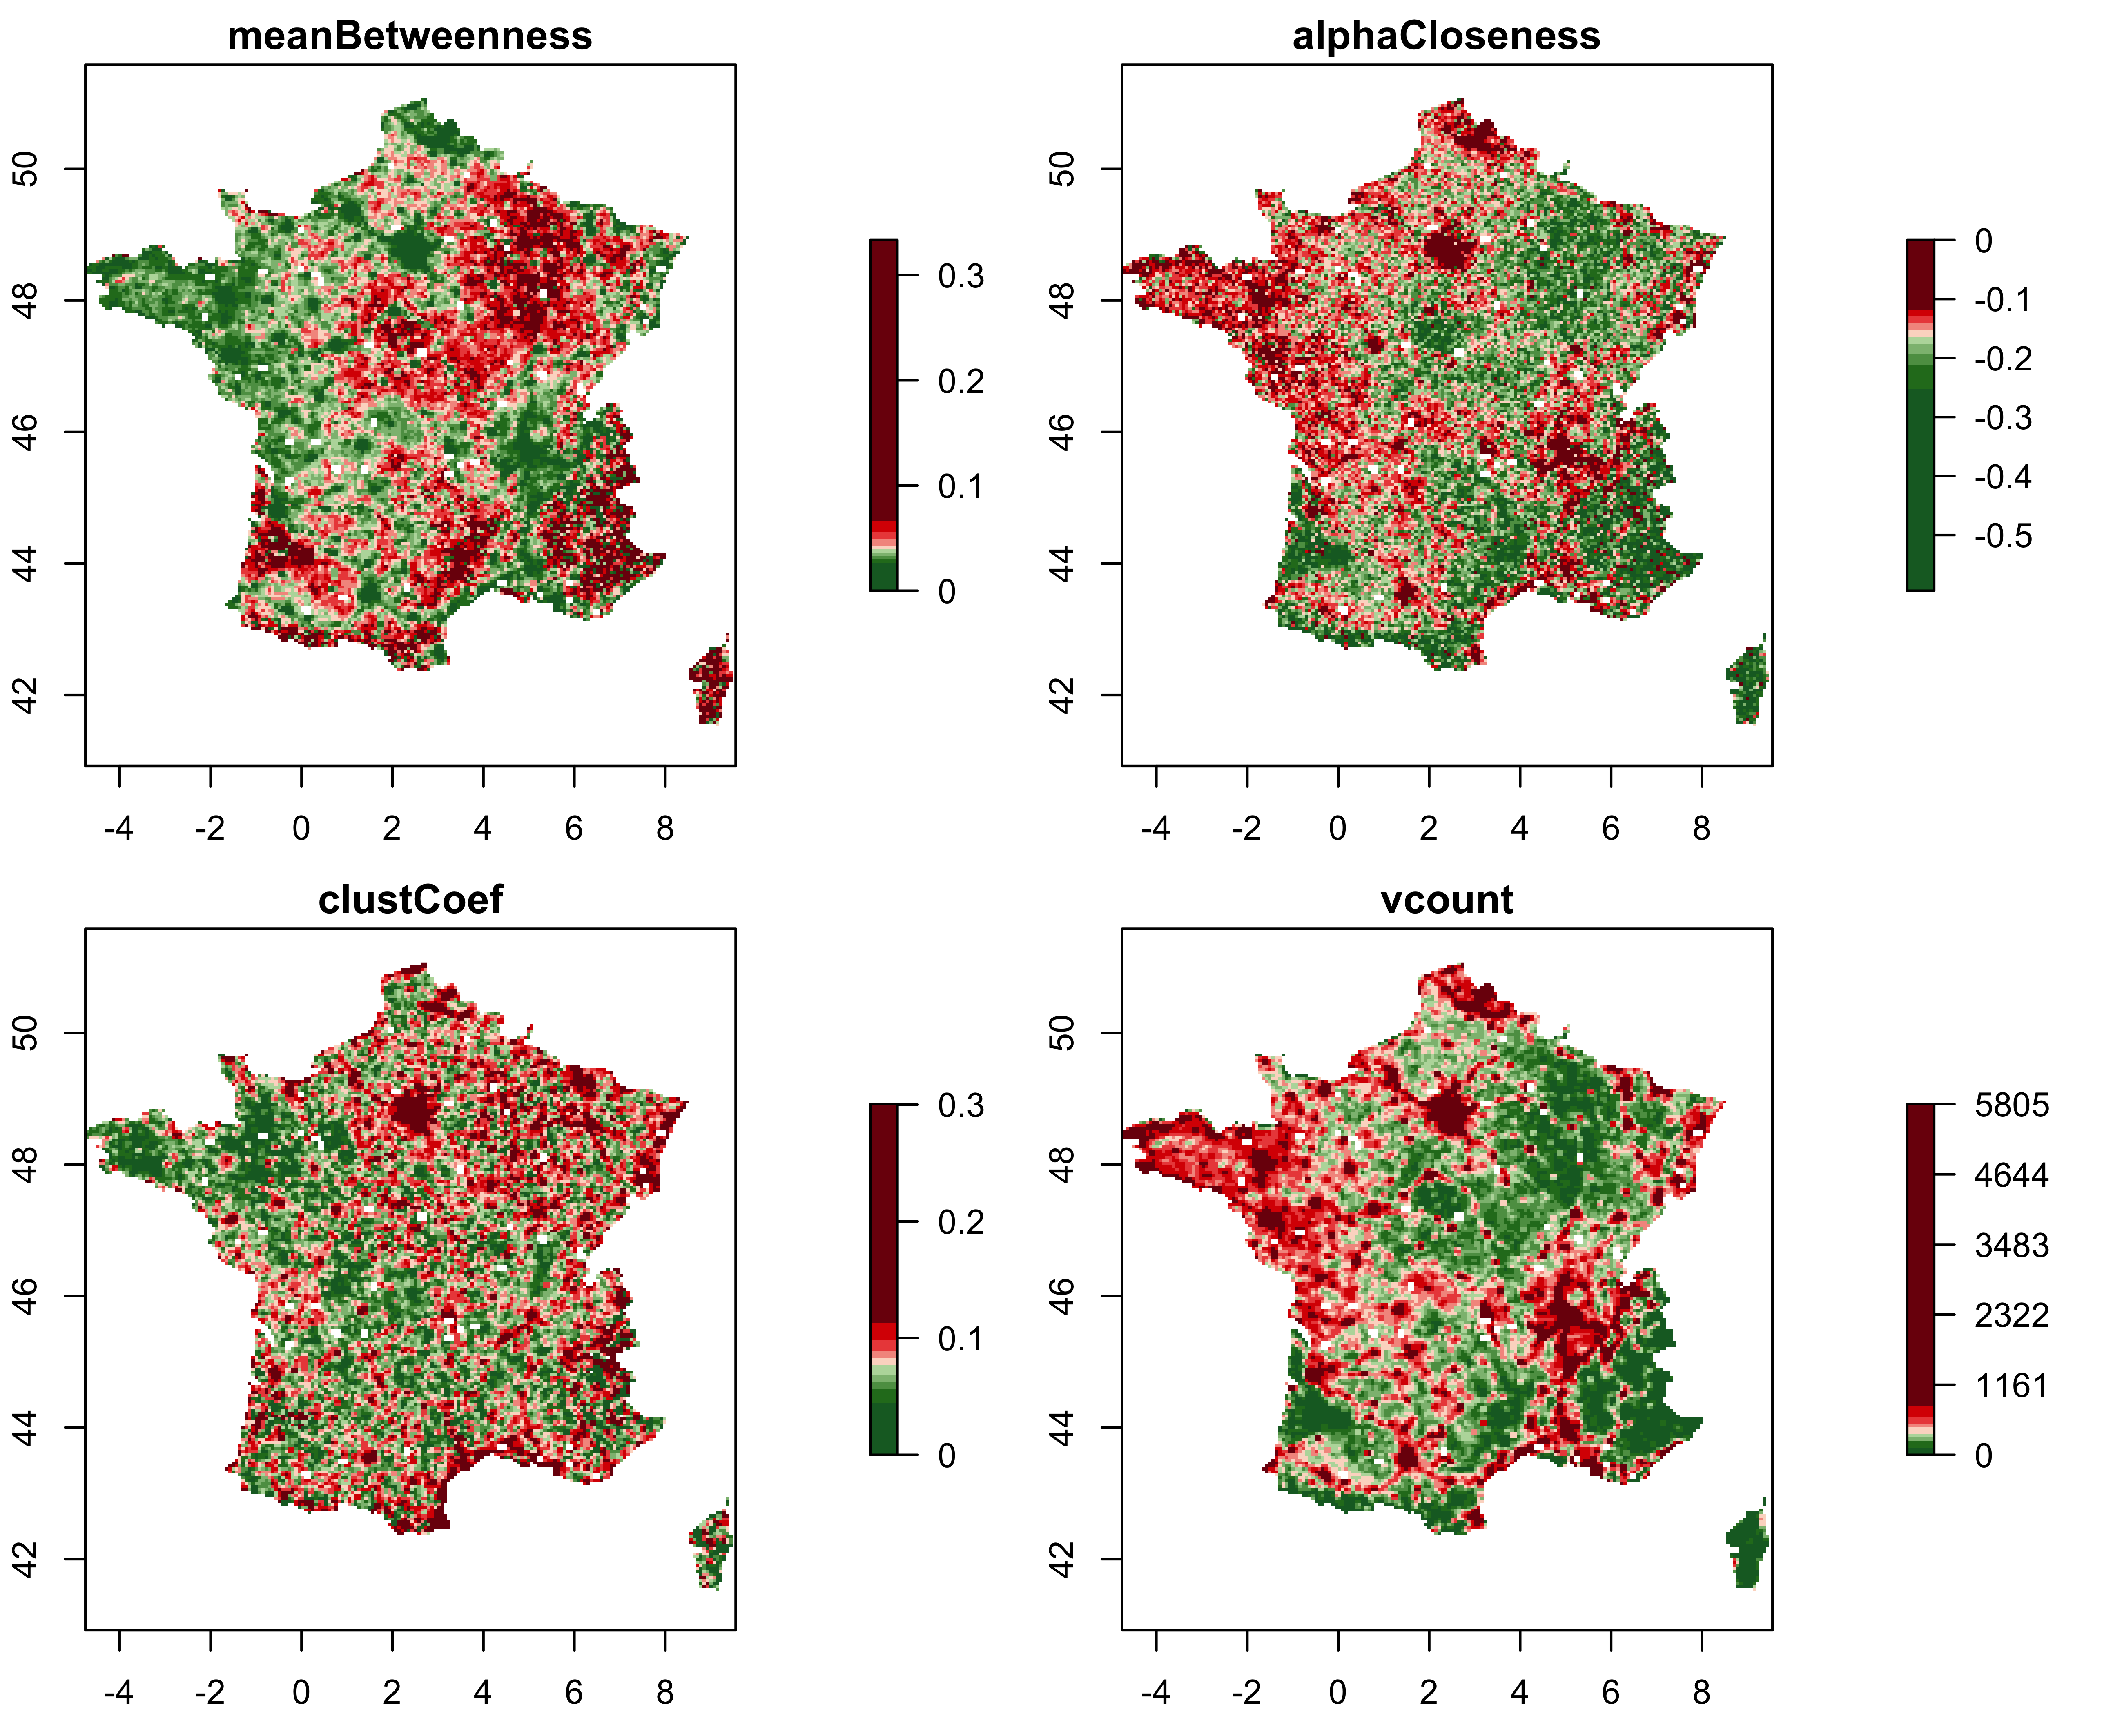
\includegraphics[width=\linewidth]{Figures/StaticCorrelations/FR_indics_network_selected_2_discrquantiles}
\caption[Empirical values of network indicators][Distribution spatiale des indicateur de réseau]{\textbf{Empirical values of network indicators.}\label{fig:staticcorrs:network}}{\textbf{Distribution spatiale des indicateur de réseau.} Nous donnons les indicateurs pour la France, en correspondance avec les indicateurs morphologiques décrits précédemment.\label{fig:staticcorrs:network}}
\end{figure}
%%%%%%%%%%%%%%%%%%%%%%%%





%%%%%%%%%%%%%%%%%%
\subsection{Effective static correlations}{Correlations Statiques Effectives et Non-stationnarité}


%%%%%%%%%%%%%%%%%%
%\subsubsection{Correlations}{Corrélations}
% short overview of overall correlations and effective dimensions
% not really needed



%%%%%%%%%%%%%%%%%%
\paragraph{Spatial Correlations}{Corrélations spatiales}


\bpar{
Pour les correlations : zones de correlation pas trop grandes, carrés de base indicateurs plus petits : Computation of urban form indicators~\cite{le2015forme} and network indicators on $l_0=10km$ side square. Computation of spatial correlation on square areas of width $\delta\cdot l_0$ (with typically $\delta = 4, \ldots , 16$) We clearly unveil the local spatial stationarity of processes.
}{
Les corrélations spatiales locales sont calculées sur des fenêtres regroupant un certain nombre d'observation, et donc de fenêtres sur lesquelles les indicateurs ont été calculés. Notons $l_0$ (qui vaut 10km dans les résultats précédents) la résolution des distributions des indicateurs. L'estimation des corrélations s'effectue alors sur des carrés de taille $\delta\cdot l_0$ (avec $\delta$ pouvant varier typiquement de 4 à 16). La valeur de $\delta$ influe directement sur le nombre d'observations, et donc la fiabilité de l'estimation. Nous montrons en Figure~\ref{fig:staticcorrs:mapscorrs} des exemples de corrélations estimées avec $\delta = 12$ dans le cas de la France. Avec 29 indicateurs, la matrice de corrélation est assez conséquente en taille, mais la dimension effective est réduite : une analyse en composante principale montre que $p=10$ capture 60\% de la variance, et la première composante capture déjà 16\%, ce qui est considérable dans un espace où la dimension avoisine les 800. On peut s'intéresser aux sous-blocs morphologique, de réseau, ou les corrélations croisées, qui exprime directement un lien entre les propriétés de la forme urbaine et celles du réseau. Par exemple, la relation entre Betweenness moyenne et hiérarchie morphologique que l'on visualise permet de comprendre la processus correspondant à la correspondance des hiérarchies : une population hiérarchisée peut induire un réseau hiérarchisé ou le sens inverse, mais elle peut également induire un réseau distribué ou celui-ci peut créer une hiérarchie de population - il faut bien comprendre en terme de correspondance et non de causalité, mais cette correspondance inform sur différents régimes urbains. Les métropoles semblent exhiber une corrélation positive dans ce cas, et des espaces ruraux négatifs. Cela suggère une très grande variété de régimes d'interaction. La variation spatiale de la première composante confirme celle-ci, ce qui révèle clairement la non-stationnarité spatiale des processus d'interaction entre formes, puisque les premiers et second moments varient dans l'espace. Nous donnons en Appendice~\ref{app:sec:staticcorrelations} d'autres exemples, pour l'ensemble de l'Europe et la Chine. Ces propriétés de non-stationnarité semblent une régularité pour l'ensemble de ces cas d'étude.
}



%%%%%%%%%%%%%%%%%%%%%%%%
\begin{figure}[h!]
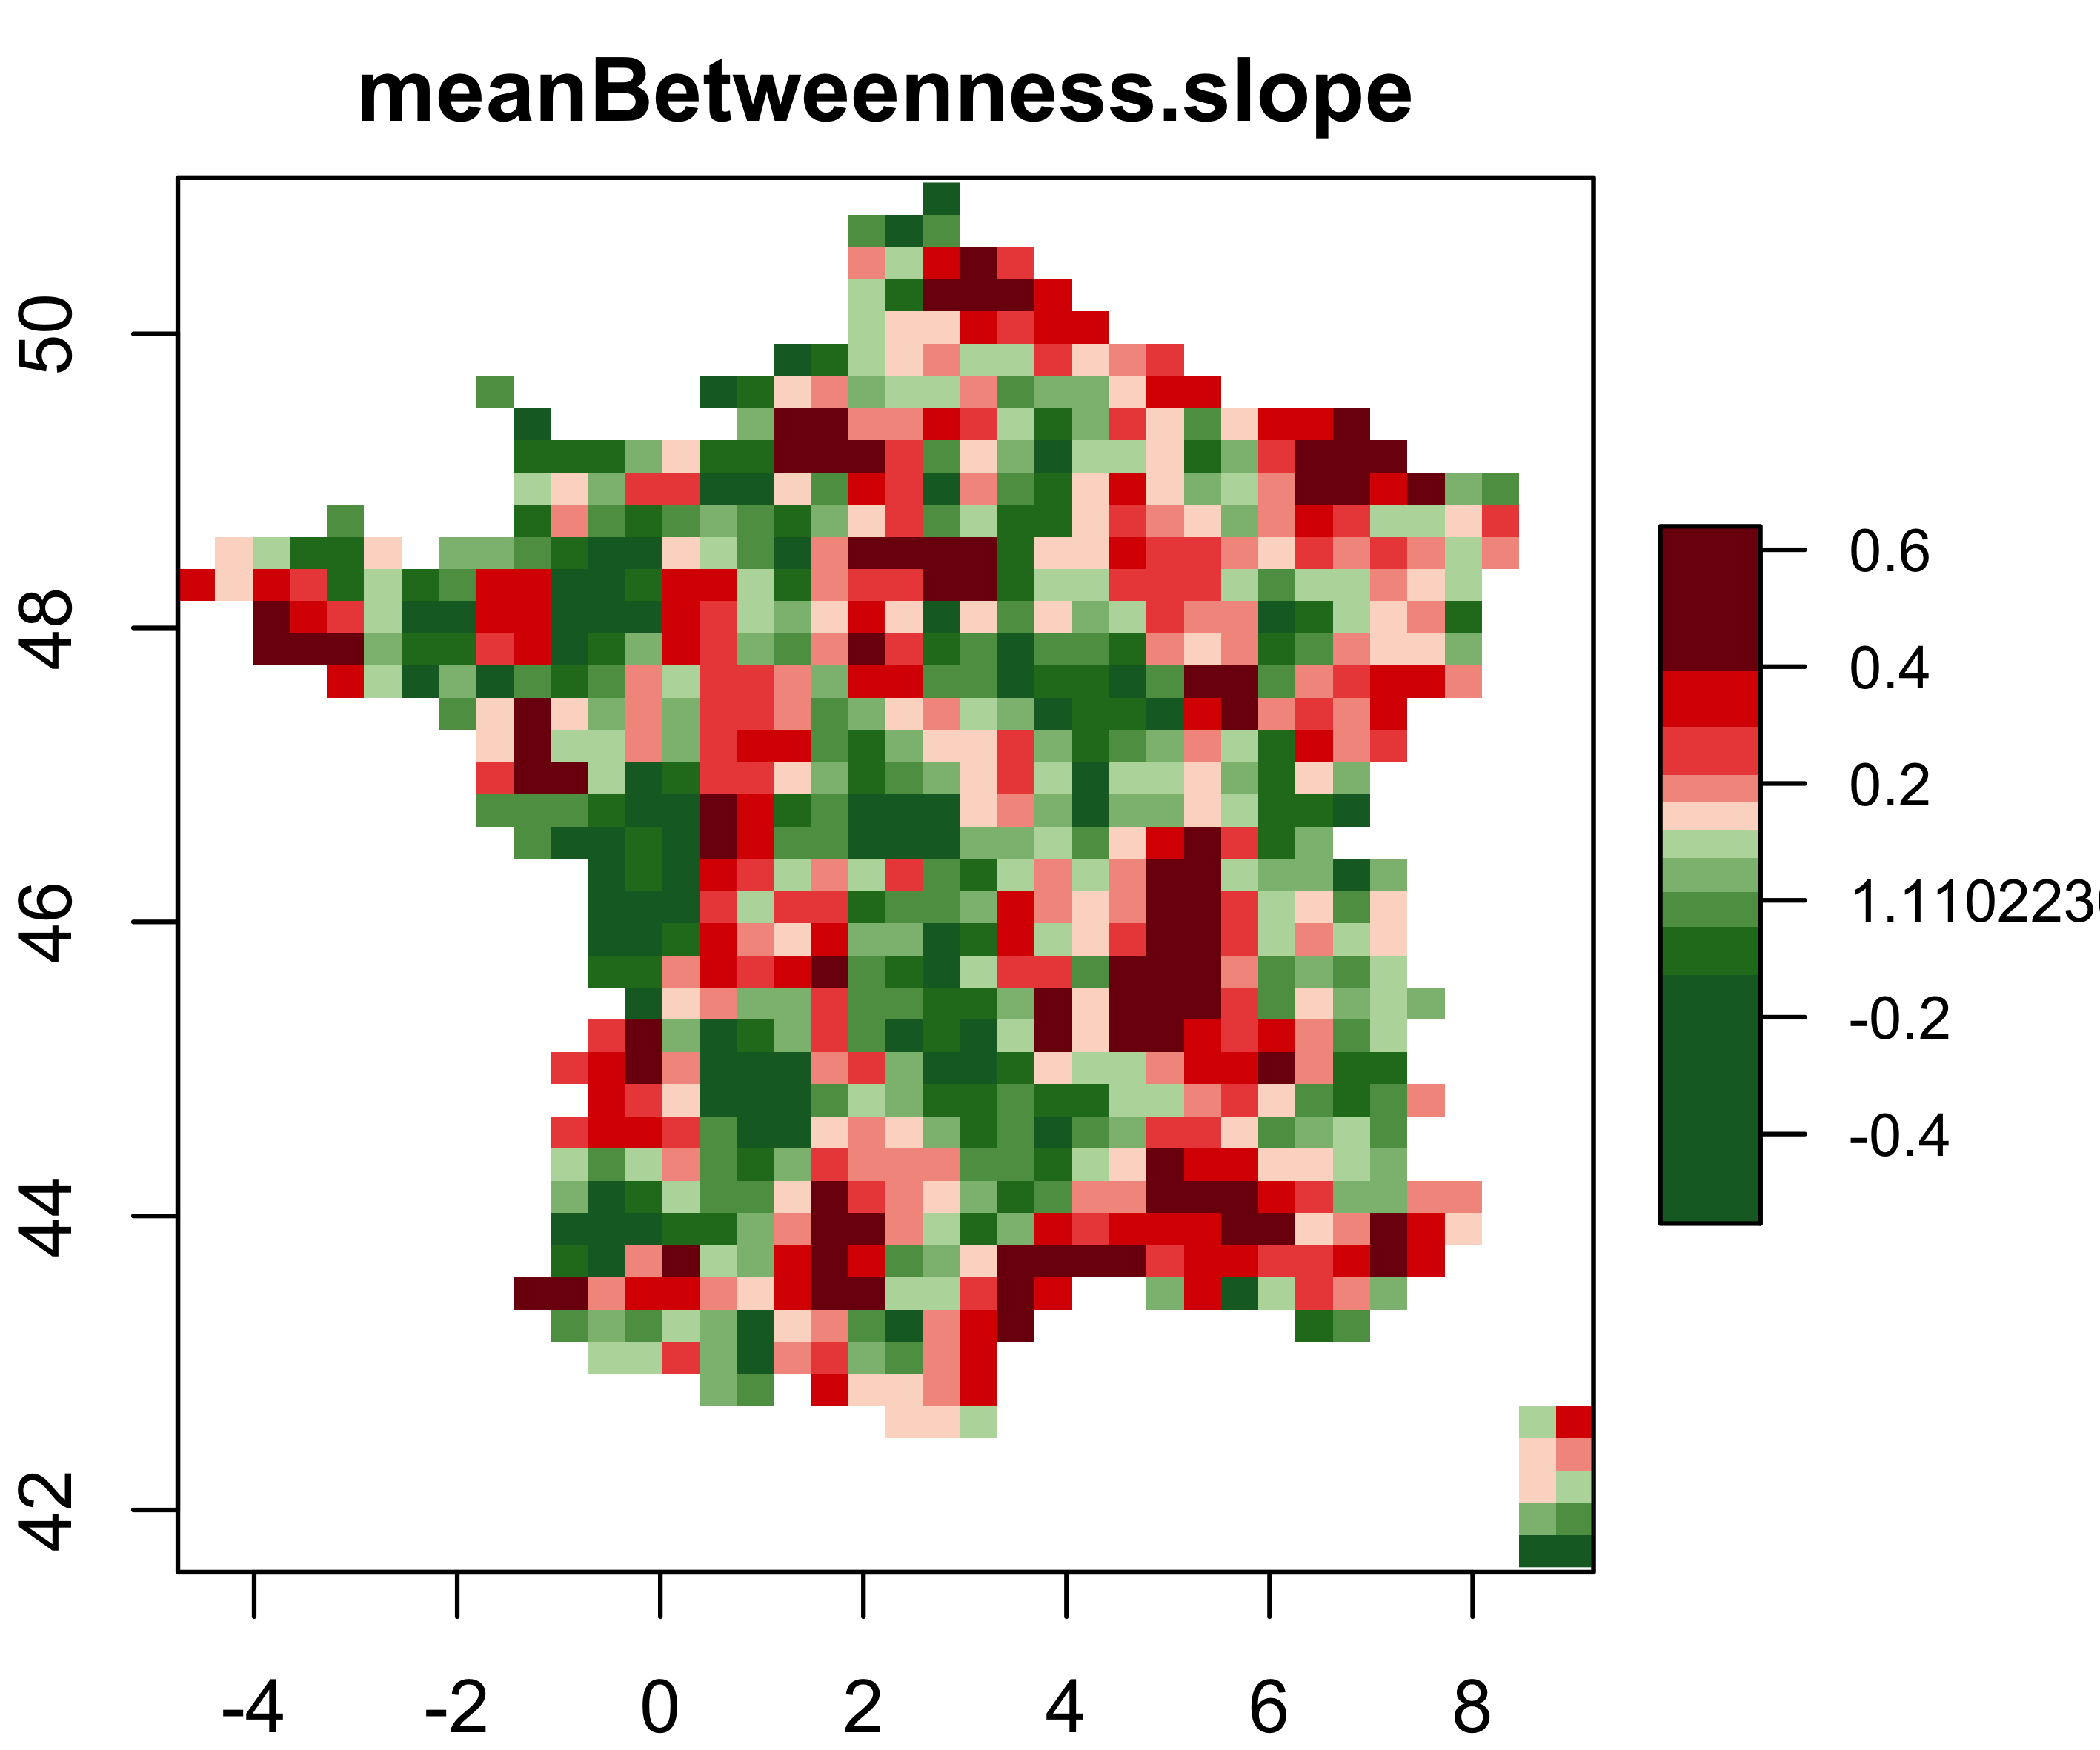
\includegraphics[width=0.48\linewidth]{Figures/StaticCorrelations/FR_corr_meanBetweenness_slope_rhoasize12}
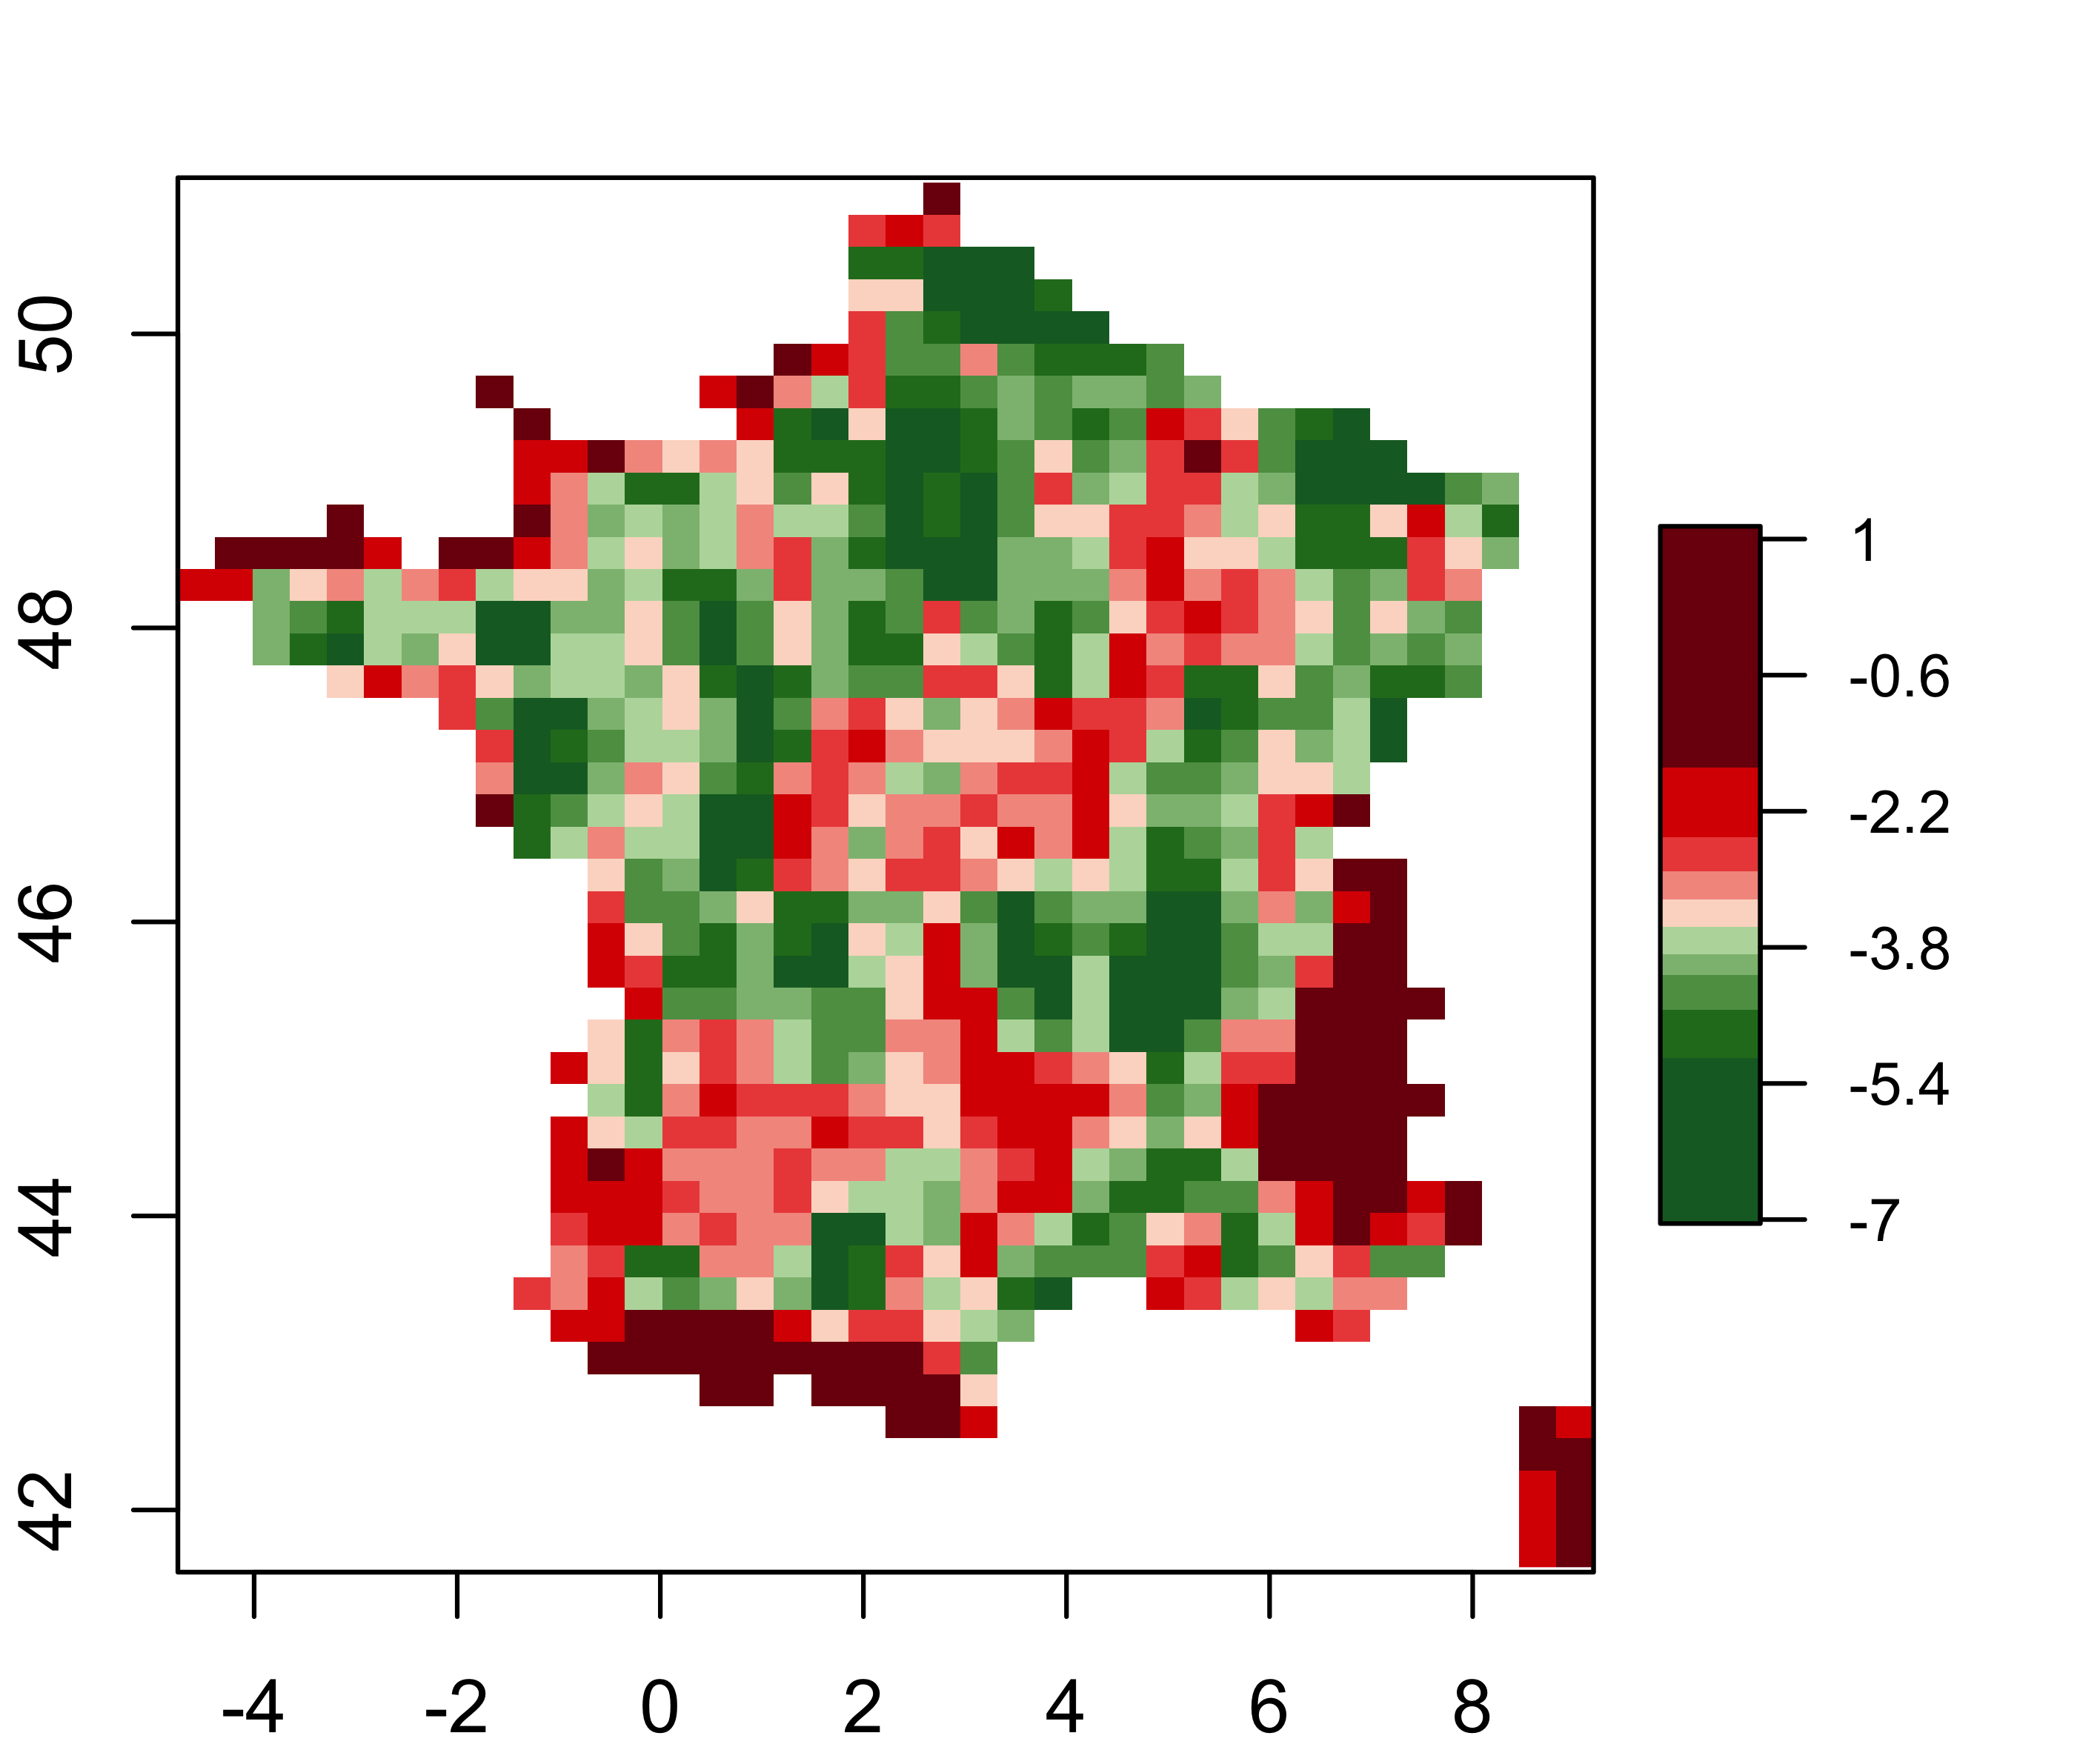
\includegraphics[width=0.48\linewidth]{Figures/StaticCorrelations/FR_corr_PCA_rhoasize12}
\caption[Spatial Correlations][Corrélations Spatiales]{Spatial Correlations\label{fig:staticcorrs:mapscorrs}}{\textbf{Exemples de corrélations Spatiales.} Pour la France, les cartes donnent $\rho\left[\bar{bw},\gamma\right]$ (gauche) et la première composante de la matrice réduite (droite).\label{fig:staticcorrs:mapscorrs}}
\end{figure}
%%%%%%%%%%%%%%%%%%%%%%%%



%%%%%%%%%%%%%%%%%%
\paragraph{Multi-scale Processes}{Nature multi-scalaire des processus}

\bpar{
$\rightarrow$ Significant variation of mean correlation with $\delta$ (Left) and of normalized confidence interval (Right) given by $\left|\rho_+ - \rho_-\right|\cdot \delta$, as bounds theoretically vary as $\sqrt{N} \sim \sqrt{\delta^2}$ : implies multi-scalarity
}{
On observe une variation significative des correlations fonction de $\delta$, qui se reflète dans la valeur moyenne de la matrice. D'abord, la distribution statistique des corrélations suit une loi similaire à une log-normale pour la morphologie seule, et plutôt normale pour le réseau et le croisement, ce qui voudrait dire que certaines zones ont des contraintes morphologiques assez fortes tandis que la forme du réseau est plutôt libre. On montre en Figure~\ref{fig:staticcorrs:corrsdistrib} ces distributions et les résultats des expériences de variation de $\delta$ pour l'Europe. On constate sur les nuages de points que les configurations où les corrélations croisées sont les plus fortes correspondent à celles où morphologique et réseau sont également fortes, confirmant l'imbrication des processus dans ce cas. L'augmentation de $\delta$ cause pour l'ensemble un décalage dans le positif, mais également un rétrécissement de la distribution, ces deux effets se traduisant par une décroissance des corrélations absolues moyennes, qui se stabilisent approximativement pour les grandes valeurs de $\delta$. Cette variation est révélateur d'un comportement multi-échelle : le changement de la taille de la fenêtre ne devrait pas influer l'estimateur si un seul processus était sous-jacent, elle devrait seulement changer la robustesse de l'estimation. Or la variation de la taille de l'intervalle de confiance normalisée, qui en théorie sous hypothèse de normalité devrait conduire $\delta\cdot \left|\rho_+ - \rho -\right|$ à être constant dans ce cas (puisque les bornes varient comme $\sqrt{N}\sim \sqrt{\delta^2}$), confirme bien cette première hypothèse. Ainsi, les processus sont à la fois non-stationnaires et multi-scalaires.
}


%%%%%%%%%%%%%%%%%%%%%%%%
\begin{figure}[h!]
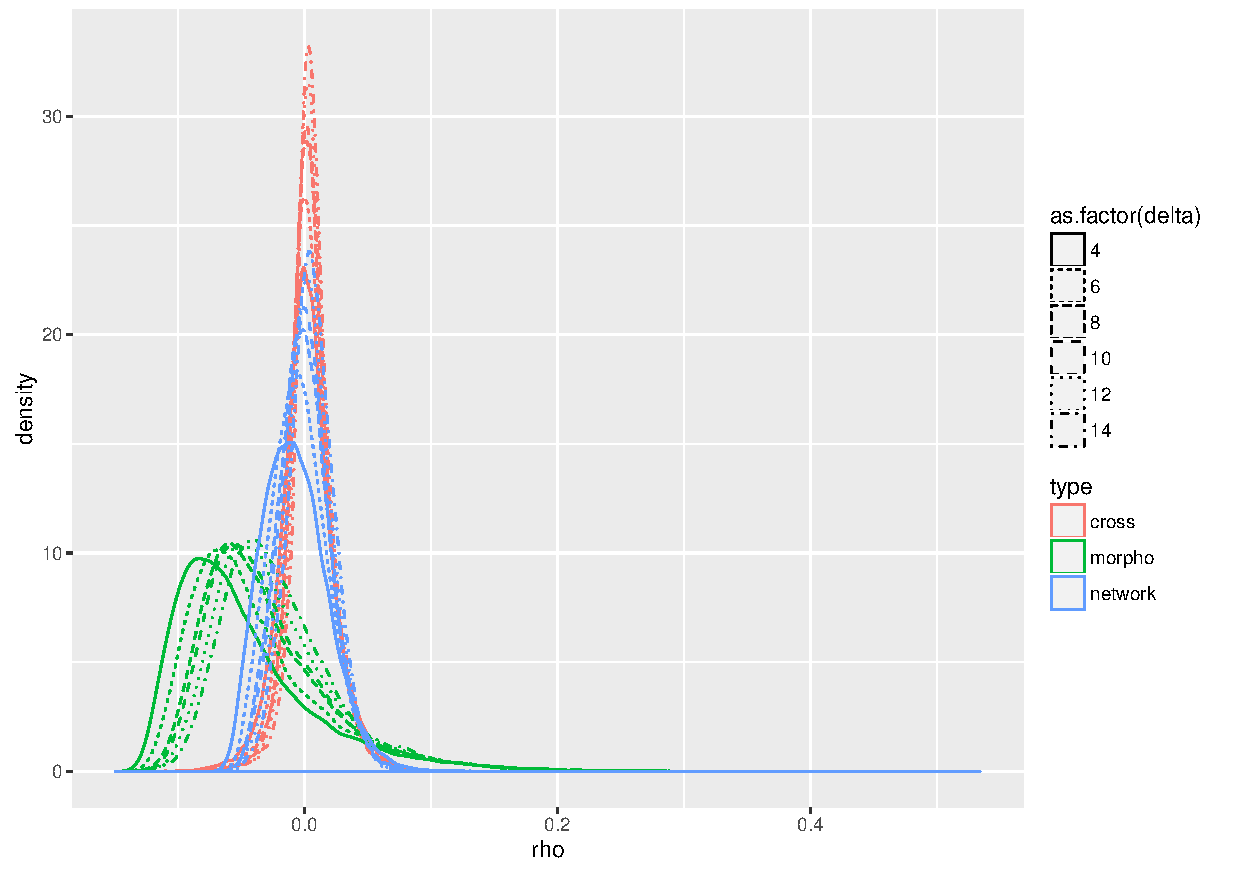
\includegraphics[width=0.48\linewidth]{Figures/StaticCorrelations/corrs-distrib_varyingdelta_bytype}
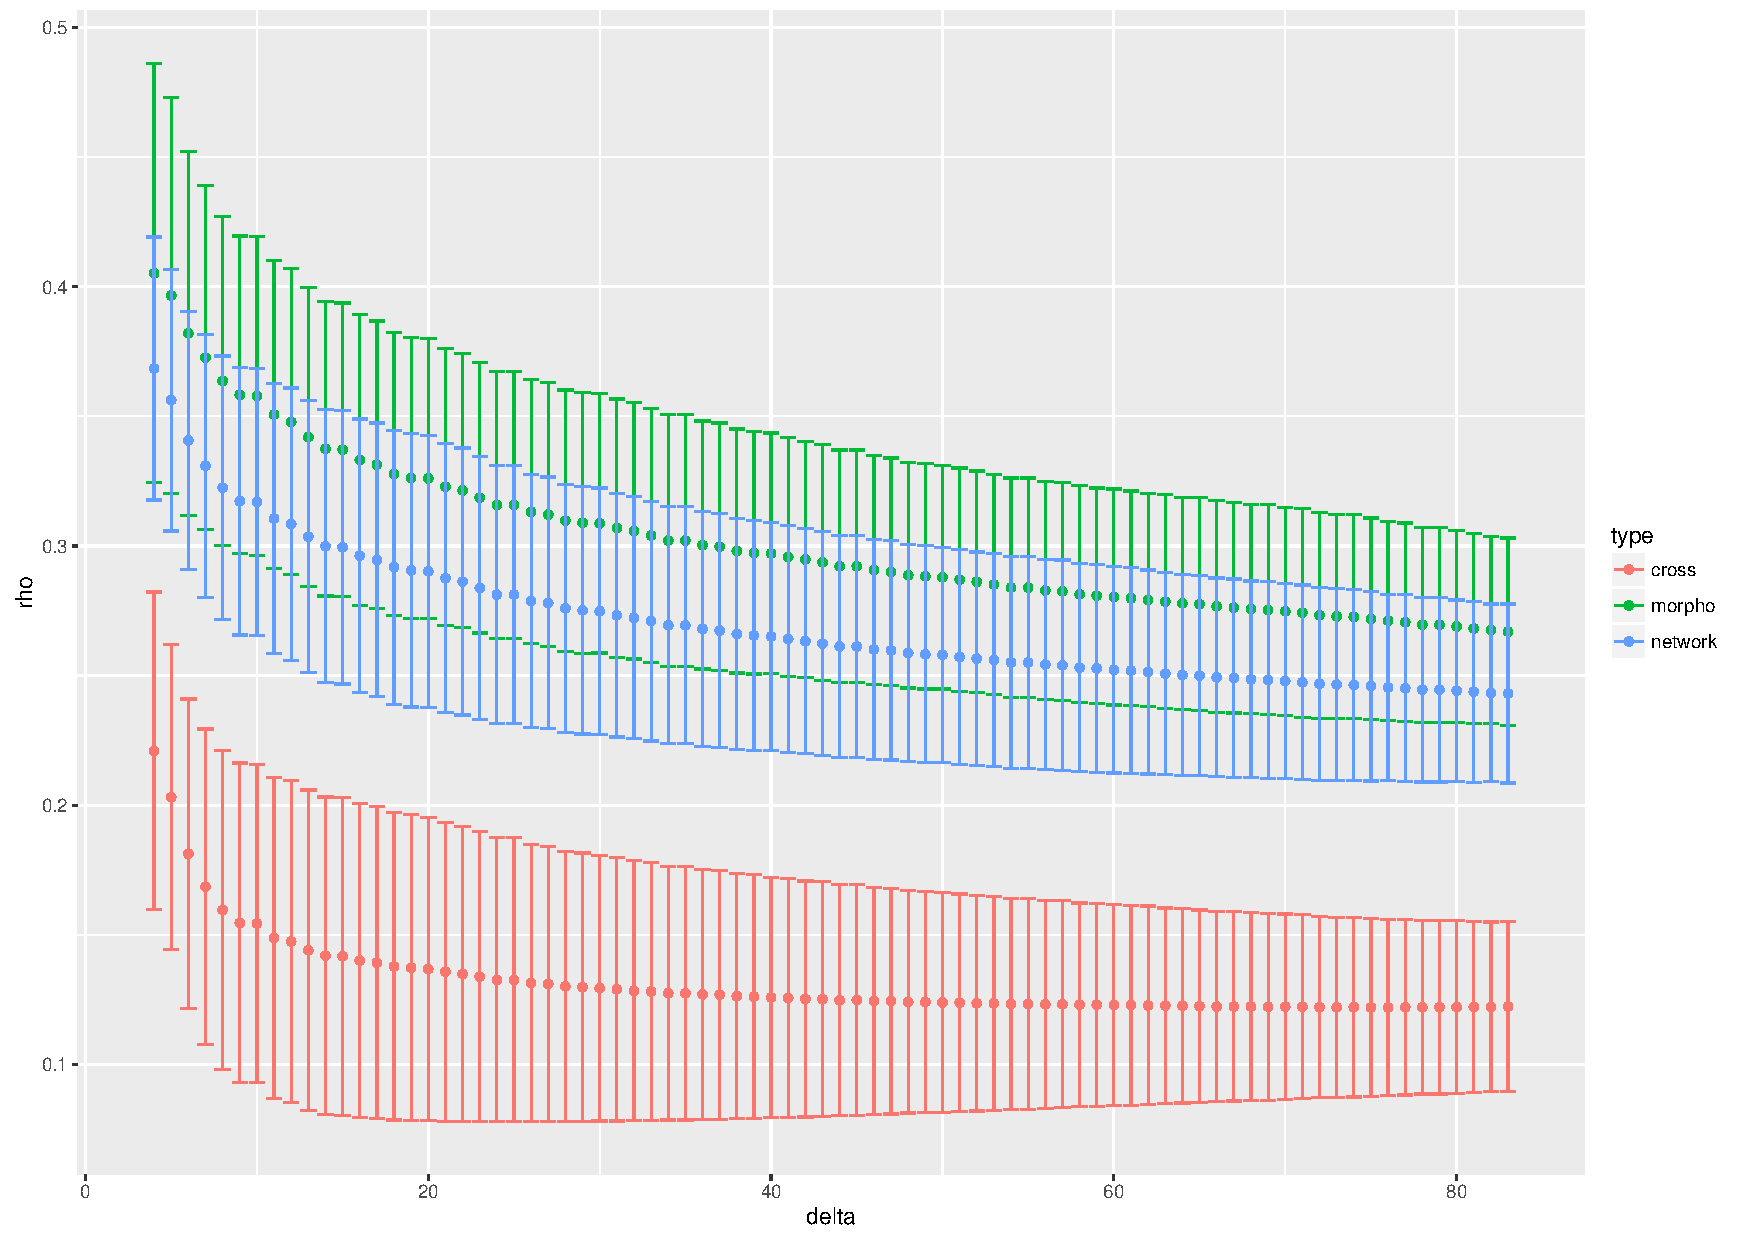
\includegraphics[width=0.48\linewidth]{Figures/StaticCorrelations/corrs-summary-meanabs_varyingdelta_bytype}\\
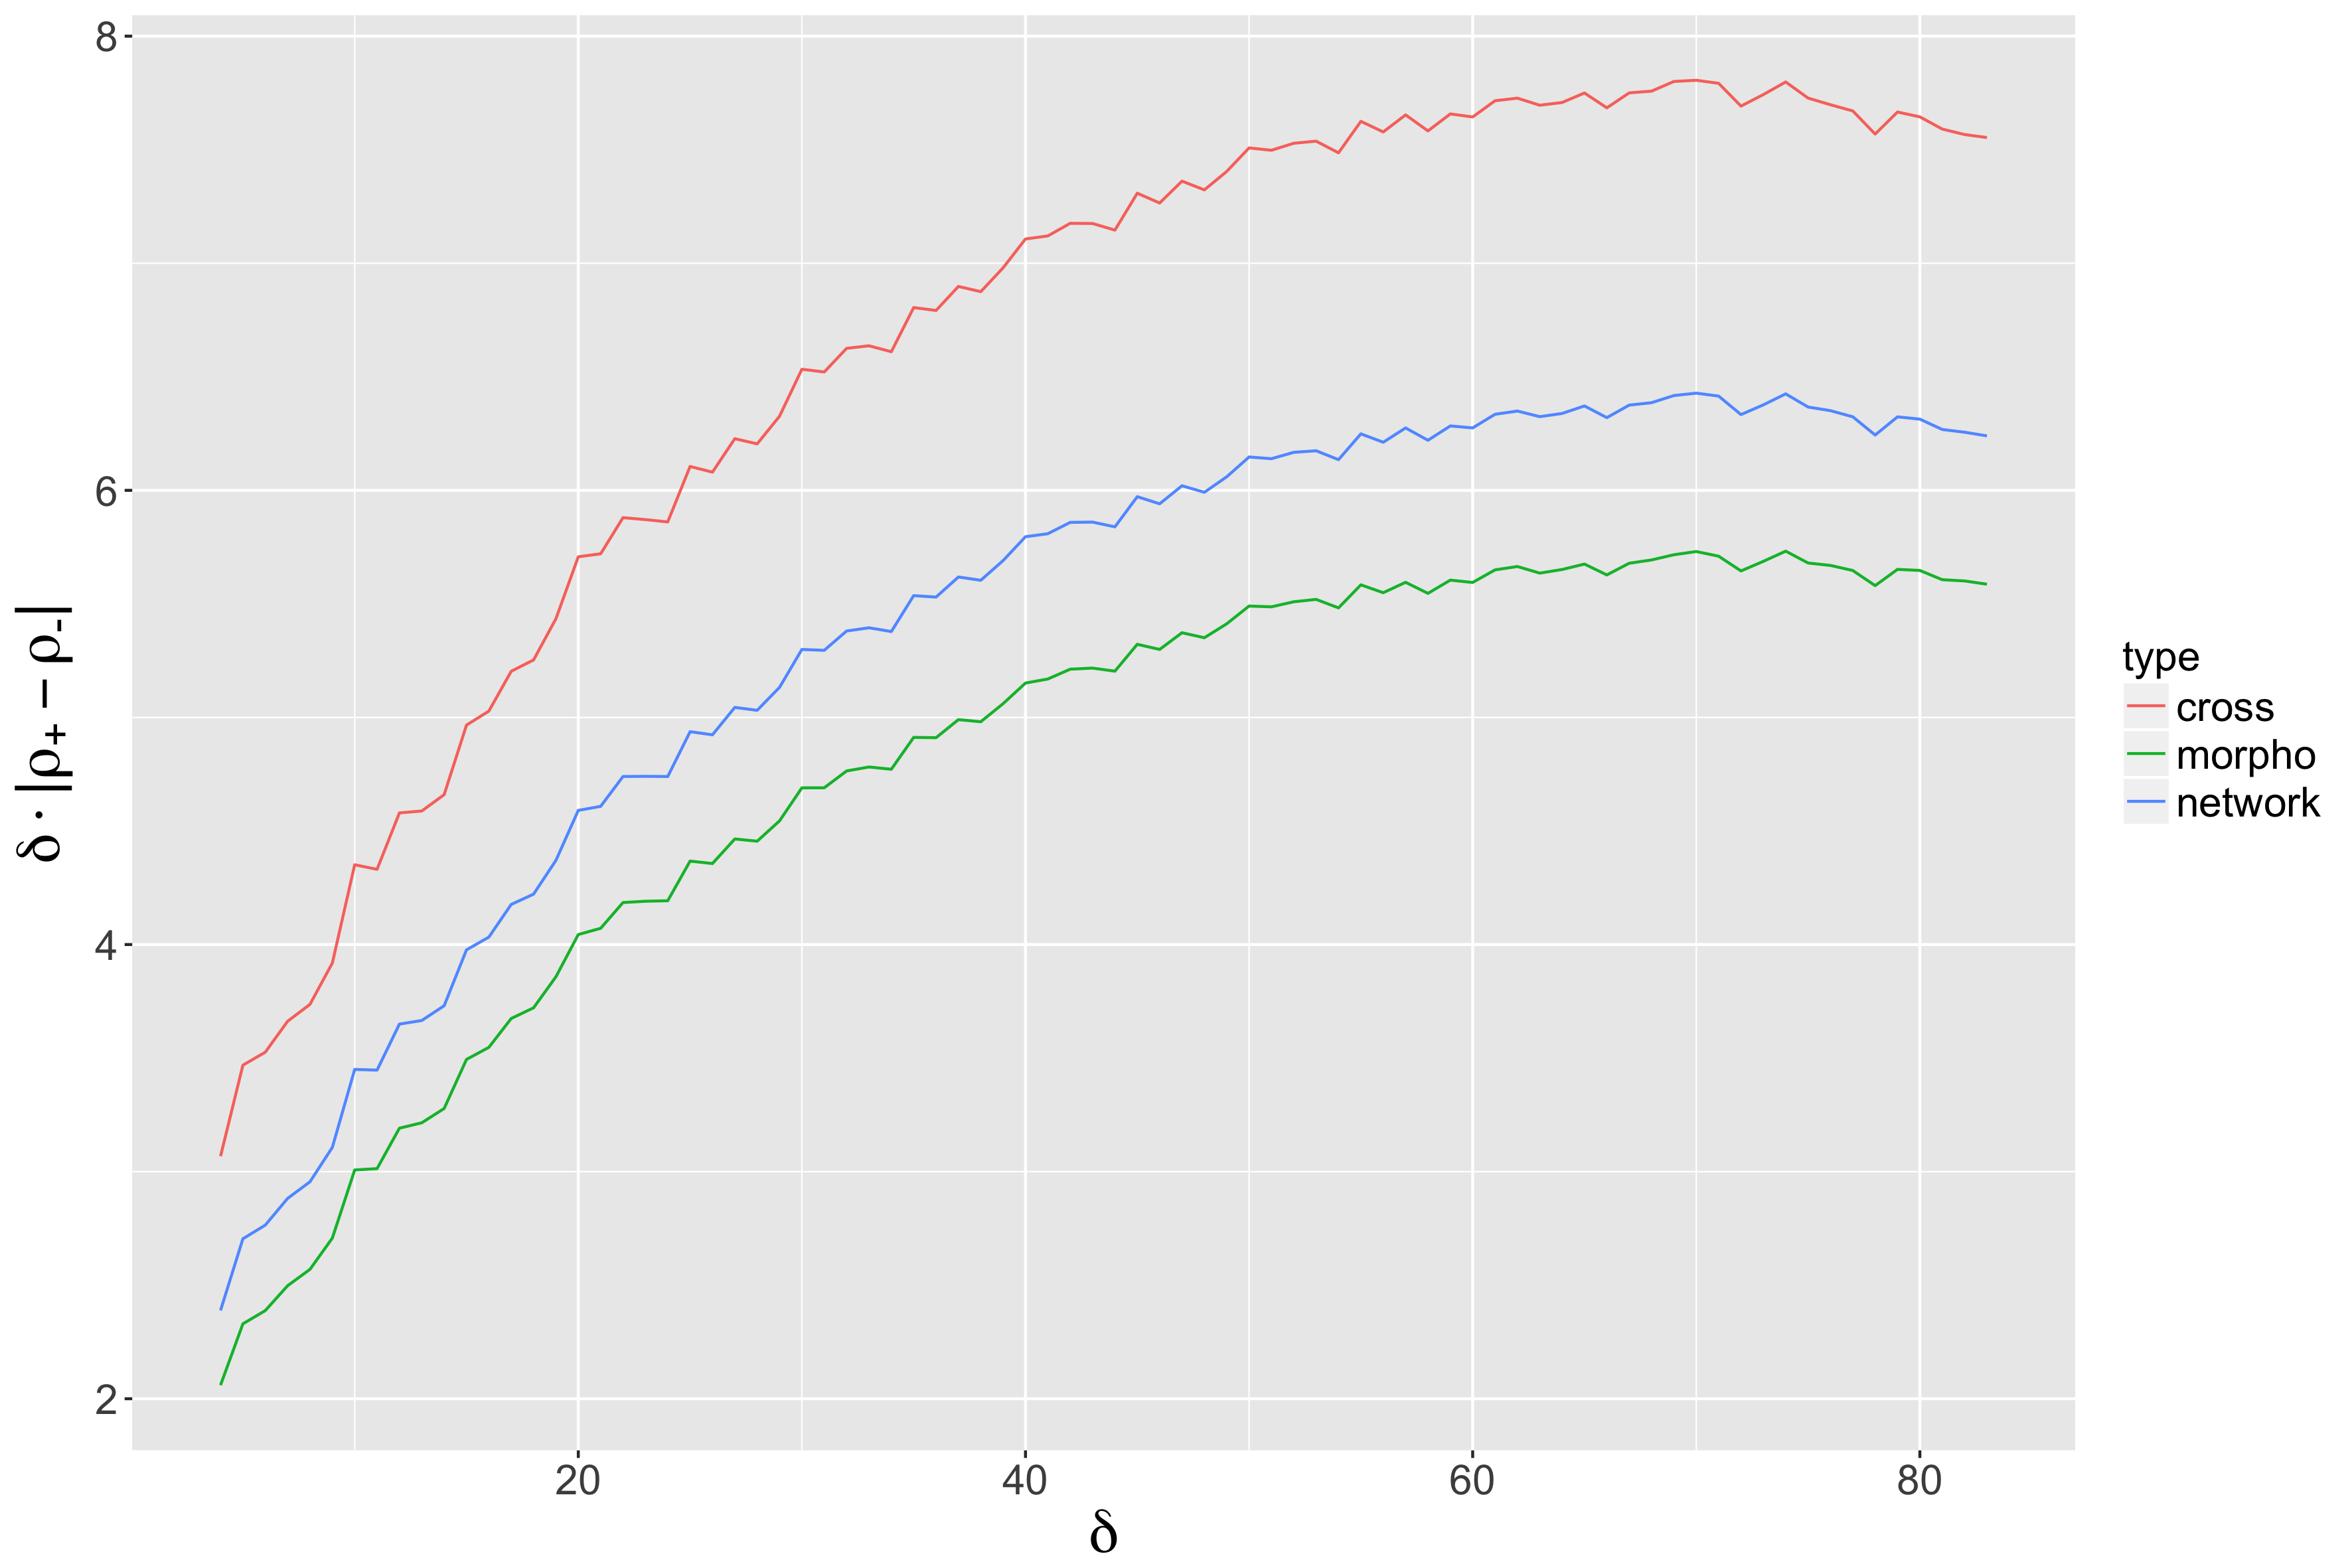
\includegraphics[width=0.48\linewidth]{Figures/StaticCorrelations/normalized_CI_delta}
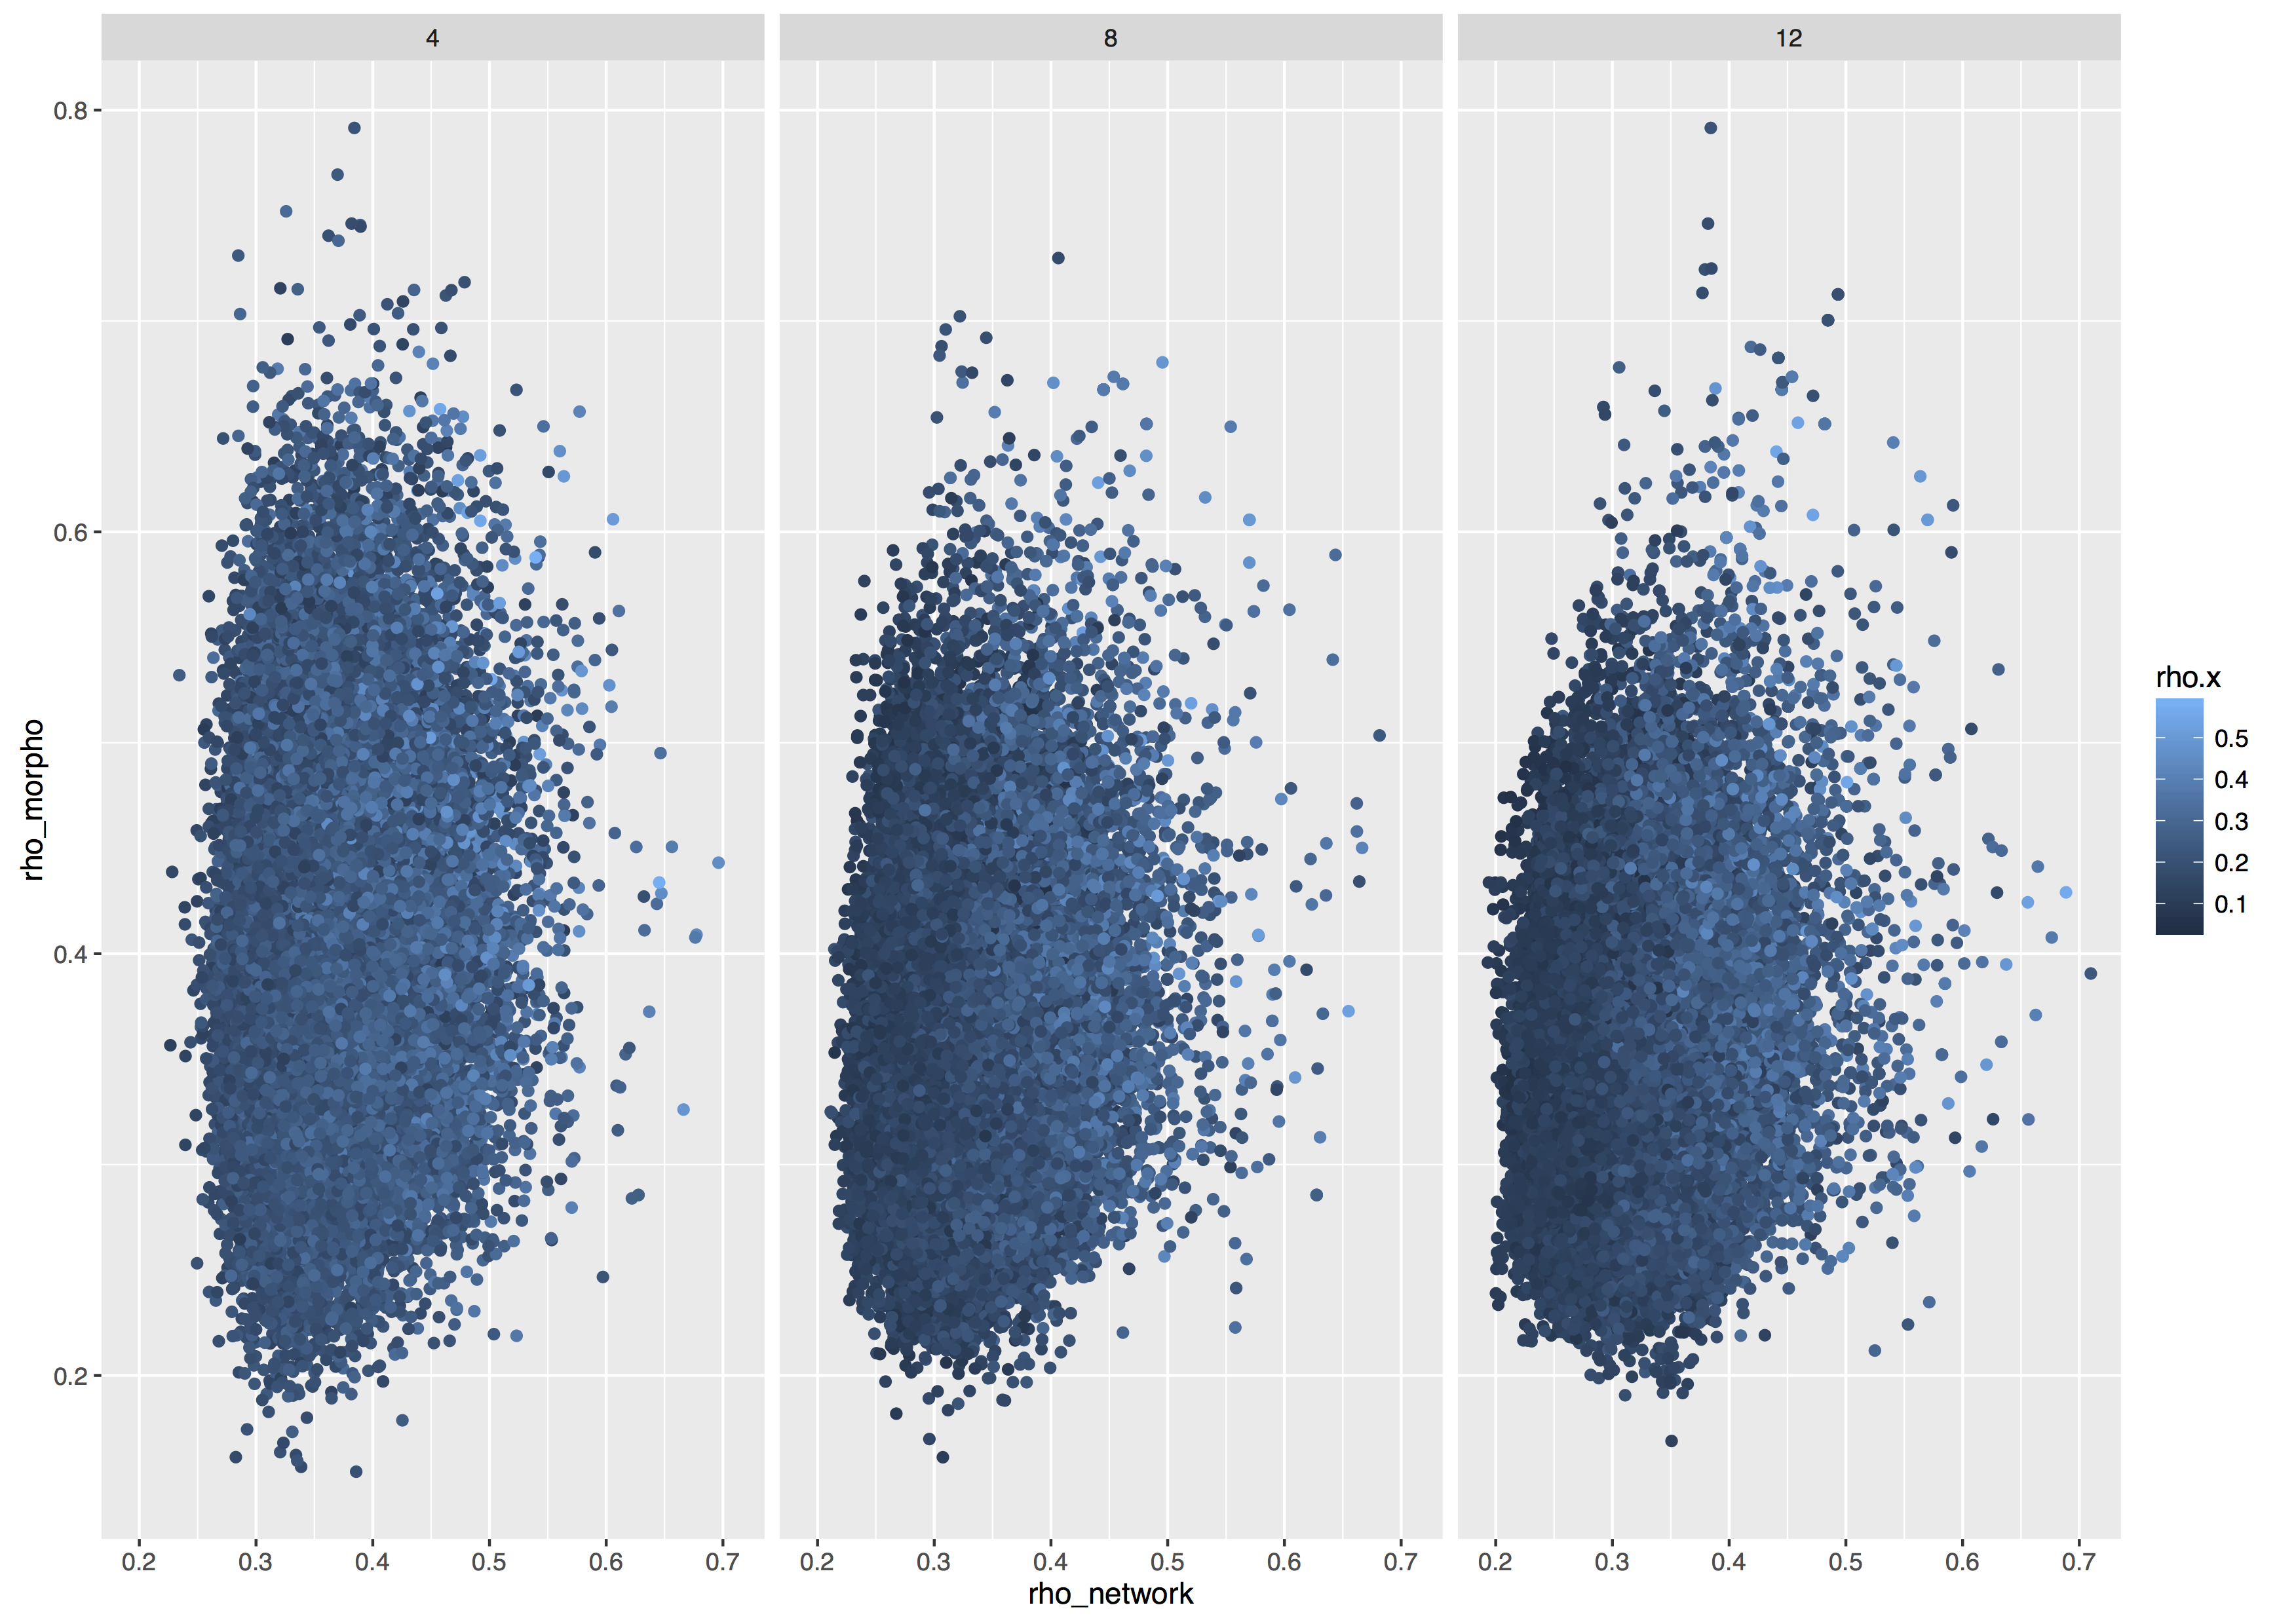
\includegraphics[width=0.48\linewidth]{Figures/StaticCorrelations/scatter_meanabs_colcross}
\caption[Variation of correlations with scale][Variation des corrélations avec l'échelle]{\textbf{Variation of correlations with scale.}\label{fig:staticcorrs:corrsdistrib}}{\textbf{Variation des corrélations avec l'échelle, pour les corrélations calculées sur l'Europe.} \textit{(Haut Gauche)} Distribution statistique des corrélations, pour les différents blocs morphologique, réseau et corrélations croisées (couleur), pour différentes valeurs de $\delta$ (type de ligne) ; \textit{(Haut Droite)} Correlations absolues moyennes et leur déviation standard, pour les différents blocs, en fonction de $\delta$ ; \textit{(Bas Gauche)} Taille de l'intervalle de confiance normalisée $\delta\cdot \left|\rho_+ - \rho -\right|$ (IC estimé par méthode de Fisher) en fonction de $\delta$ ; \textit{(Bas Droite)} Correlation absolues moyennes pour le réseau en fonction de la morphologie, niveau de couleur donnant la corrélation croisée, pour différentes valeur de $\delta$.\label{fig:staticcorrs:corrsdistrib}}
\end{figure}
%%%%%%%%%%%%%%%%%%%%%%%%



%%%%%%%%%%%%%%%%%%
%\paragraph{Optimal Scales}{Echelles optimales}


%\bpar{
%We also compute the optimal bandwidth for a GWR PCA~\cite{harris2011geographically}. We beware to sample data accordingly to avoid local colinearity :\cite{wheeler2007diagnostic} colinearity in GWR
%}{

%}





%%%%%%%%%%%%%%%%%%
\subsubsection{Spatial non-stationarity and non-ergodicity}{Non-stationnarité spatiale et non-ergodicité}


\paragraph{Formalization}{Formalisation}

\bpar{
We propose to formalize our empirical findings. Let $Y_i\left[\vec{x},t\right]$ a spatio-temporal stochastic process. We showed following assumptions:
\begin{enumerate}
\item Local spatial autocorrelation is present and bounded by $l_{\rho}$ (in other words the processes are continuous in space) : at any $\vec{x}$ and $t$, $\left|\rho_{\norm{\Delta \vec{x}} < l_{\rho}}\left[Y_i (\vec{x}+\Delta \vec{x},t), Y_i (\vec{x},t) \right]\right| > 0$.
\medskip
\item Processes are locally parametrized : $Y_i = Y_i\left[\alpha_i\right]$, where $\alpha_i (\vec{x})$ varies with $l_{\alpha}$, with $l_{\alpha} \gg l_{\rho}$ and weakly locally stationary in space.
\medskip
%\item Spatial correlations between processes have a sense at an intermediate scale $l$ such that $l_{\alpha}\gg l \gg l_{\rho}$.
%\item Processes covariance stationarity times scale as $\sqrt{l}$.
%\item Local ergodicity is present at scale $l$ and dynamics are locally chaotic.
\item Processes are multi-scalar : since $\rho(\delta = \infty) > \rho (\delta = 0 )$, a necessary non-linear correction on processes spatial averages in correlation computation is present.
% add computation in supplementary materials / papers. -> later
\end{enumerate}
}{
Formalisons les conclusions empiriques obtenues. Soit $Y_i\left[\vec{x},t\right]$ un processus stochastique spatio-temporel. Nous avons alors les hypothèses suivantes :
\begin{enumerate}
\item L'autocorrelation spatiale locale existe en dessous d'une échelle minimale $l_0$ (en d'autres termes le processus est continu dans l'espace) : pour tout $\vec{x}$ et $t$, on a $\left|\rho_{\norm{\Delta \vec{x}} < l_0}\left[Y_i (\vec{x}+\Delta \vec{x},t), Y_i (\vec{x},t) \right]\right| > 0$.
\item Les processus sont localement paramétrisés : $Y_i = Y_i\left[\alpha_i\right]$, où $\alpha_i (\vec{x})$ varie à l'échelle $l_{\alpha}$, avec $l_{\alpha} \gg l_0$ et est localement stationnaire dans l'espace.
\item Les processus sont multi-scalaires : comme $\rho(\delta = \infty) > \rho (\delta = 0 )$, une nécessaire correction non-linéaire sur les moyennes spatiales des processus est présente dans le calcul des corrélations.
\end{enumerate}
}


\paragraph{On global non-ergodicity}{Sur la non-ergodicité globale}

\bpar{
Analytical Deductions
1. \textbf{Regimes of temporal correlations.} Let assume local ergodicity in $\vec{x}_0$ at scale $\delta \cdot l_0$ (reasonable with urban growth and network extension in recent times). The Ergodic theorem implies that $\exists \mathcal{T}$ such that

\[<Y_i (t) >_{\norm{\vec{x}-\vec{x}_0} < \delta\cdot l_0} = <Y_i (\vec{x}_0)>_{t\in \mathcal{T}}\] 

With spatial stationarity, $<Y_i>_{\vec{x}_0}=<Y_i>_{\vec{x}_1}$, thus $\mathcal{T}$ must be constant to be invariant by translation. By contraposition and (2), processes have different dynamical characteristics.
% if translate in a given direction, looses a small part, must be compensated by the area translated by delta (overlap), thus must be constant.
2. \textbf{Global non-ergodicity.} Let $X_k$ a partition of space into local areas. We have $<\cdot>_x = \sum_k w_k <\cdot>_{x_k} =_{(1)} \sum_k w_k <\cdot>_{\mathcal{T}_k} $. On the other hand, global ergodicity would give $<\cdot>_t = <\cdot>_{\mathcal{T}} = \sum_k w_k <\cdot>_{\mathcal{T}}$ and $\sum_k w_k \left(<\cdot>_{\mathcal{T}} - <\cdot>_{\mathcal{T}_k}\right) = 0$. Being true on each subset implies $\mathcal{T}=\mathcal{T}_k$, what contradicts (1).
}{
Nous proposons d'esquisser un lien entre les propriétés de non-stationnarité et la non-ergodicité globale des systèmes, qui est un aspect essentiel postulé par la Théorie Evolutive~\cite{pumain2012urban}, conduisant à discuter les interprétation universelles des systèmes urbains proposées par les théories du Scaling~\cite{bettencourt2007growth}. Nous suggérons que la non-stationnarité spatiale est reliée d'une part à différentes échelles de temps impliquées, et d'autre part à une non-ergodicité globale, sous l'hypothèse de stationnarité et d'ergodicité locale. Cette dernière parait raisonnable, au sens ou un régime local se manifestera de manière aléatoire sur ses différentes instances locales dans le cas d'indicateurs effectivement stochastiques à cette échelle (on pourra considérer les résultats de simulation de~\ref{sec:densitygeneration} pour se donner une idée). Empiriquement, la croissance urbaine et du réseau assez récente, rapide et étendue, laisse penser qu'on devrait être dans un cas analogue. Supposons ergodicité locale en $\vec{x}_0$ à l'échelle $\delta \cdot l_0$ à laquelle nous estimons les corrélations. Alors le théorème ergodique fournit un échantillonnage temporel $\mathcal{T}$ tel que 
\[
<Y_i (t) >_{\norm{\vec{x}-\vec{x}_0} < \delta\cdot l_0} = <Y_i (\vec{x}_0)>_{t\in \mathcal{T}}
\]
En se plaçant en un autre point $\vec{x}_1$ assez loin, la stationnarité spatiale devrait impliquer $<Y_i>_{\vec{x}_0}=<Y_i>_{\vec{x}_1}$ et $\mathcal{T}$ sera similaire pour garder invariance par translation. Par contraposition comme on a montré la non-stationnarité, les processus ont ainsi nécessairement des caractéristiques dynamiques différentes. Concernant la non-ergodicité globale, soit $X_k$ une partition de l'espace en zones locales. On a  $<\cdot>_x = \sum_k w_k <\cdot>_{x_k} = \sum_k w_k <\cdot>_{\mathcal{T}_k} $. Mais d'autre part, l'ergodicité globale impliquerait que  $<\cdot>_t = <\cdot>_{\mathcal{T}} = \sum_k w_k <\cdot>_{\mathcal{T}}$ et donc $\sum_k w_k \left(<\cdot>_{\mathcal{T}} - <\cdot>_{\mathcal{T}_k}\right) = 0$. Pour que cette relation soit vraie sur la totalité des sous-ensembles, il est nécessaire que $\mathcal{T}=\mathcal{T}_k$, ce qui contredit la propriété montrée précédemment, et le système global est nécessairement non-ergodique. Ces résultats dépendent des hypothèses théoriques, mais nous postulons qu'ils devraient rester vrais de manière empirique vu les suggestions de la Théorie Evolutive.
}






%%%%%%%%%%%%%%%%%%
\subsubsection{Discussion}{Discussion}


\paragraph{Universality}{Universalité}

\bpar{
In \cite{10.1371/journal.pone.0107042} density grids for other countries across the world are provided\footnote{available at \url{http://www.worldpop.org.uk/}}. The analysis may be repeated to other regions of the world, to compare the correlation regimes and test if urban system properties stay the same. We can expect different regimes for the United States compared to Europe for example, but the discrepancy needs still to be investigated~\cite{bretagnolle2010comparer}.
}{
Des grilles de densité de population existent pour l'ensemble des régions du monde, comme par exemple celles fournies par~\cite{10.1371/journal.pone.0107042}\footnote{disponibles à \url{http://www.worldpop.org.uk/}}. L'analyse peut être répétée pour d'autres régions, pour comparer les régimes de corrélations et tester si les propriétés des systèmes urbains restent les mêmes, en gardant à l'esprit les difficultés liées aux différences de qualité dans les données. On peut s'attendre à des régimes très différents pour les Etats-Unis en comparaison à l'Europe par exemple~\cite{bretagnolle2010comparer}, mais la différence se doit d'être étudiée quantitativement.
}



\paragraph{Further Developments}{Développements}


\bpar{
We show the regional nature of network-territories interactions, in particular the non-ergodicity of urban systems on \textbf{the interaction these components}. No direct results on time dynamics, but indirect : spatio-temporal processes do not have same speed and react/diffuse differently. Still points to explore :
\begin{itemize}
\item variable correlations areas (size and shape in space)
\item same work on cities population/train network data, which are also dynamical databases : extrapolation of ergodicity parameters ?
\item correlations of returns : link between $\rho\left[\Delta_t Y\right]$ and $\rho\left[\Delta_x Y\right]$ (more difficult : if pure local ergodicity, $\exists$ a permutation making the correspondance) % may be difficult to identify 
\item Link between $\Delta_{\delta}\rho (\delta)$ and process derivatives ?
\end{itemize}
}{
Nous avons montré empiriquement la non-stationnarité des interactions entre forme urbaine et forme de réseau, qui suggère la non-ergodicité du système urbain concernant l'interaction entre ces composantes. Nous n'extrayons pas de résultats directs sur les dynamiques par ces analyses statiques, mais pouvons postuler des résultats indirects : les processus spatio-temporels n'ont pas les mêmes vitesses et réagissent et diffusent différemment. Certains développements de cette étude serait potentiellement intéressants. La recherche d'échelle locales, c'est à dire avec une fenêtre d'estimation adaptative en taille et forme pour les corrélations, permettrait de mieux comprendre la façon dont les processus influent localement sur leur voisinage. Le critère validation de la taille resterait à déterminer : il peut s'agir comme ci-dessus de portée optimale pour des modèles locaux. La question de l'ergodicité doit également être explorée sur des bases dynamiques, en comparant les échelles de temps et d'espace d'évolution des processus, ou plus précisément les corrélations entre les variations dans le temps $\rho\left[\Delta_t Y\right]$ et celles dans l'espace $\rho\left[\Delta_x Y\right]$, mais la question de l'existence de base assez fines dans le temps paraît problématique. L'étude d'un lien entre $\Delta_{\delta}\rho (\delta)$ est les dérivées des processus est également une piste pour obtenir des informations indirectes sur la dynamique à partir des données statiques.
}








\stars




